\documentclass[12pt,a4paper,twoside]{article}
\usepackage{graphicx} % Required for inserting images
\usepackage[
backend=biber,
style=apa
]{biblatex}
\usepackage{amsmath}
\usepackage{float}
\usepackage{caption}
\usepackage[english]{babel}
\usepackage{breqn}
\usepackage{xcolor}
\usepackage{csquotes}
\usepackage[a4paper, margin=1in]{geometry}
\usepackage{setspace}
\usepackage{graphicx}
\usepackage{hyperref}
\usepackage{booktabs}
\usepackage{siunitx}
\usepackage[toc,page]{appendix}

%%%%%%%%%%%%%% Third level subsection %%%%%%%%%%%%%%%%%%%
\usepackage{titlesec}

\titleclass{\subsubsubsection}{straight}[\subsection]

\newcounter{subsubsubsection}[subsubsection]
\renewcommand\thesubsubsubsection{\thesubsubsection.\arabic{subsubsubsection}}
\renewcommand\theparagraph{\thesubsubsubsection.\arabic{paragraph}} % optional; useful if paragraphs are to be numbered

\titleformat{\subsubsubsection}
  {\normalfont\normalsize\bfseries}{\thesubsubsubsection}{1em}{}
\titlespacing*{\subsubsubsection}
{0pt}{3.25ex plus 1ex minus .2ex}{1.5ex plus .2ex}

\makeatletter
\renewcommand\paragraph{\@startsection{paragraph}{5}{\z@}%
  {3.25ex \@plus1ex \@minus.2ex}%
  {-1em}%
  {\normalfont\normalsize\bfseries}}
\renewcommand\subparagraph{\@startsection{subparagraph}{6}{\parindent}%
  {3.25ex \@plus1ex \@minus .2ex}%
  {-1em}%
  {\normalfont\normalsize\bfseries}}
\def\toclevel@subsubsubsection{4}
\def\toclevel@paragraph{5}
%\def\toclevel@paragraph{6}
\def\toclevel@subparagraph{6}
\def\l@subsubsubsection{\@dottedtocline{4}{7em}{4em}}
\def\l@paragraph{\@dottedtocline{5}{10em}{5em}}
\def\l@subparagraph{\@dottedtocline{6}{14em}{6em}}
\makeatother

\setcounter{secnumdepth}{4}
\setcounter{tocdepth}{4}
%%%%%%%%%%%%%%%%%%%%%%%%%%%%%%%%%%%%%%%%%%%%%%%%%%%%%%%%
% Keywords command
\providecommand{\keywords}[1]
{
  \small	
  \textbf{\textit{Keywords---}} #1
}
%%%%%%%%%%%%%%%%%%%%%%%%%%%%%%%%%%%%%%%%%%%%%%%%%%%%%%%%
% % Add abstract environment to book style
% \newenvironment{abstract}%
% {\cleardoublepage \null \vfill \begin{center}%
% 		\bfseries \abstractname \end{center}}%
% {\vfill\null}
%%%%%%%%%%%%%%%%%%%%%%%%%%%%%%%%%%%%%%%%%%%%%%%%%%%%%%%
% Set font to Times New Roman
%\usepackage{mathptmx}

% Set double spacing
\doublespacing


\addbibresource{bibliography.bib}

\title{The PnL Drivers of Long-Short Trading Strategies}
% \author{Ioannis Paraskevopoulos, Fernando Celaya}
\date{\today}

\begin{document}
\pagestyle{empty}
\begin{titlepage}
  \begin{figure}
    \centering
    
\includegraphics[width=0.3\linewidth]{assets/logo-comillas.png}
  \end{figure}
  \centering
  \Large 
  Degree in Business Administration \\ Bachelor's Final Thesis\\[36px]
  \Huge 
  The PnL Drivers of Long-Short Trading Strategies\\
  \Large
  \raggedright
  \vspace*{\fill}
  Author: Fernando Celaya\\
  Supervisor: Ioannis Paraskevopoulos\\
  \today

\end{titlepage}
\newpage

\begin{abstract}
  This work improves the performance of a cointegration-based pairs trading strategy by refining its implementation and expanding its asset universe. Through detailed backtesting, the strategy's overall performance and long and short legs are analyzed separately and compared to the market and a Johansen cointegration based benchmark. The strategy demonstrates strong risk-adjusted performance, with low negative beta to the market. Its performance drivers are analyzed through a five factor model and it is found to be driven primarily by the size factor and the Idiosyncratic Equity Volatility Premium. A secondary regression identifies high market capitalization, high profitability as per the $ROC$, and high valuation as per the $BTM$ and $EVEBITDA$ of its traded assets as other key performance drivers. 
\end{abstract}
\keywords{Pairs-trading, Cointegration, Performance analysis, Profit drivers, Factor model, Idiosyncratic Equity Volatility Premium}
\newpage

\section*{Acknowledgements}
I would like to express my deepest gratitude to my supervisor, Ioannis Paraskevopoulos, not only for his invaluable guidance and support throughout this project but also for sharing with me his passion for quantitative finance and illuminating my way in this incredibly interesting field. I would also like to thank Alvaro Guerrero for his generosity lending an impeccable starting point for this thesis and his deep support whenever it was needed. 
\newpage

\thispagestyle{empty}
\tableofcontents
\newpage

\thispagestyle{empty}
\listoffigures
\listoftables
\newpage


\pagestyle{plain}
\clearpage
\pagenumbering{arabic}
\section{Introduction}
\subsection{Overview of long-short trading strategies}
When someone has a positive expectation for the performance of an asset in the market, the simplest way to profit from it is to buy that asset. If the asset is a stock for example one could buy shares of that stock. If the expectation was correct, when that asset goes up in price those shares can be sold and the difference in price is kept as profit. Buying an asset is generally called "going long".

But what if one expects a negative performance for some asset? It is also possible to profit from these views by doing the opposite. The share can be borrowed and sold in the market, to be later bought at a lower price and keeping the difference as profit. This is generally called "going short" on an asset.

There are a few reasons why going short on an asset is however not as straightforward as going long. For one, even though the borrowing of shares is a very streamlined process nowadays it is still more cumbersome than simply buying the asset. Furthermore, it entails borrowing costs for the time while the position is open and it is also riskier. In addition to that, while long positions have a maximum loss of 100\% -- when the price of the asset goes to 0 -- short positions can lose more than 100\%. If the price triples for example and one is to close the position, one must buy the asset spending three times the amount of money originally received when selling the borrowed shares, leading to a loss of 200\%. In order to prevent this situation and to make sure that the shares are always given back, short positions -- like leveraged positions --  can also lead to margin calls, materializing our losses when there are sudden price movements in the market.

Allowing for short positions however also has some benefits. It allows asset managers or traders to profit also from negative views on some assets, not only from positive ones. In more technical terms, by removing the constraint stating that all positions must be positive, the new universe of possible positions is much greater with better options. This can be seen very clearly in the asset allocation problem, where by removing the short selling constraint the efficient frontier is expanded and better portfolios can be formed. 

One of the possible formulations for the optimal portfolio allocation problem is the following:

$$
\begin{aligned}
    \text{min} \quad & \sigma_p^2 = \mathbf{w}^\top \Sigma \mathbf{w} \\
    \text{s.t.} \quad & \mathbf{w}^\top \mathbf{r} = \mu \\
    & \mathbf{w}^\top \mathbf{1} = 1 \\
    & \mathbf{w} \geq 0
\end{aligned}
$$


Where $\sigma_p^2$ is the portfolio variance, $w$ is the vector of portfolio weights, $\Sigma$ is the matrix of asset covariances, $r$ is the vector of asset returns and $\mu$ is the target portfolio return. 

The second constraint is the no-leverage constraint, assuming that the portfolio is self-financed, while the third constraint is the no-short-selling constraint, where all portfolio weights are forced to be positive. 
The difference between including and not including the last constraint can be observed in the following figure, where the portfolio problem has been solved for different target returns for each of the two portfolios. 

\begin{figure}[h]
    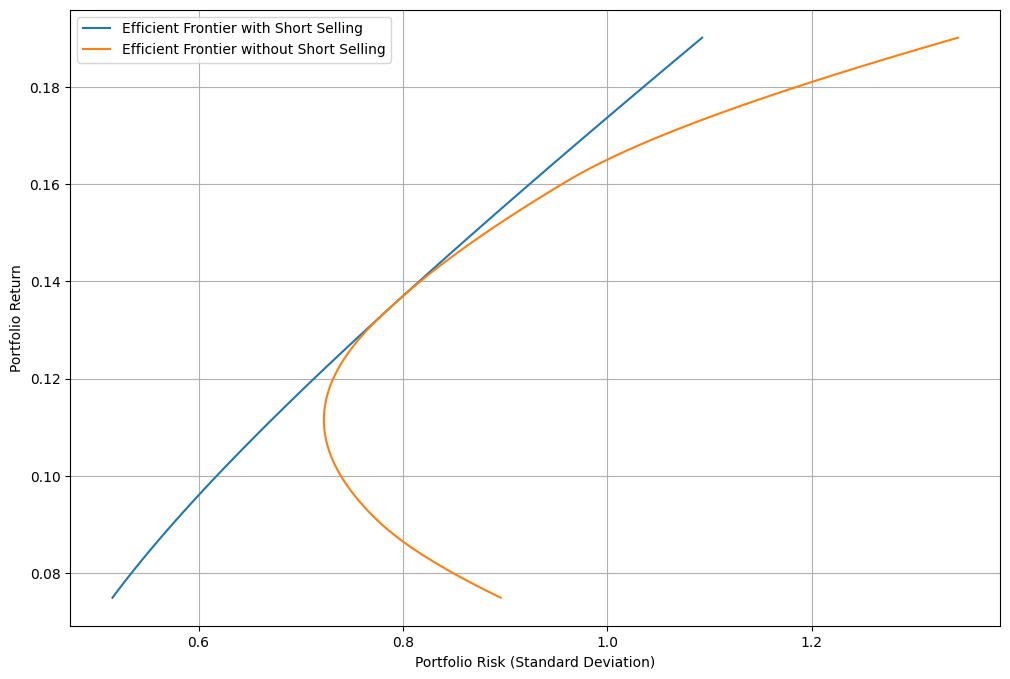
\includegraphics[width=\linewidth]{assets/efficient-frontier-comparison.png}
    \caption{Comparison of efficient frontiers with and without short selling constraint}
    \label{fig:efficient-frontier-comparison}
\end{figure}

As it can be clearly seen in \autoref{fig:efficient-frontier-comparison}, for a given risk level, the optimal portfolio without the short selling constraint has expected returns equal or greater than the optimal portfolio with the constraint. 

Any strategy that allows for both the buying and selling of assets is thus called a long-short trading strategy, and there are many such strategies with different purposes and characteristics. The strategy that will be studied here is a pairs-trading strategy.
\subsubsection{Pairs-trading strategies}
These strategies were first developed by a group of traders at Morgan Stanley in 1985 under the leadership of Nunzio Tartaglia and they follow a very simple principle. If two assets move very similarly, but onw thinks for some reason that one of them is going to outperform the other, then a long position is entered in that one and a short position is entered in the other one. That way, the general movement of the market can be takan out of the position, and the profit of the trade will only depend on the difference in movement between the two assets, and not on the market movements affecting both assets. 
This can be seen more clearly with a samll extension to the $CAPM$ model, where asset specific component for the return are included.
\begin{equation}
    r_A=r_f+\beta_A(r_M-r_f)+ r_S^A+ \epsilon_A
\end{equation}
\begin{equation}
    r_B=r_f+\beta_B(r_M-r_f)+ r_S^B+ \epsilon_B
\end{equation}


A position can be chosen for both assets with position sizes $\Delta_A$ and $-\Delta_B$ and $\Delta_A\beta_A=\Delta_B\beta_B$ so that
\begin{equation}
    r_P=\Delta_Ar_A-\Delta_Br_B=(\Delta_A-\Delta_B)r_f + \Delta_A r_S^A - \Delta_B r_S^B + \epsilon_P
\end{equation}
As it can be seen, the market or non specific part of the returns disappears, with the portfolio returns depending mainly on the specific part of the returns of each of the assets. Or more specifically, on the difference between these components. 

Having a strategy with returns independent to that of the market can be very attractive, as this strategy can in theory provide positive reutrns regardless of the behaviour of the market. Furthermore, by combining several sources of uncorrelated returns -- as none of them are correlated to the market any longer -- one can achieve a very well diversified portfolio with a great return to risk relationship. 

The question of how one can find two such assets which move very similarly requires a bit more attention. As outlined by \cite{review_statistical_arbitrage} there are many approaches studied in the litereature to finding such pairs. These include the Distance approach, Time series approach, Stochastic control approach, Copula approach, Principal Component Analysis approach, etc. The one that will be relevant here hawever is one method which relies on the idea of cointegration. Suppose there are two or more time series $X_1, X_2$, with order of integration $d$. That is, by differentiating the time series $d$ times the resulting time series is covariance-stationary -- its mean and autocovariance are constant through time and its variance is finite. The two time series are cointegrated if there exists a linear combination of the two through which the resulting time series has an oder of integration of less than $d$. 

Note that this is similar to the removal of the market returns explained above but even more powerful. If enough cointegrated return time series are found, one could combine them having a portfolio with returns with a constant mean. Assured profits!

\subsection{Significance of understanding PnL drivers}
Understanding the Profit and Loss (PnL) drivers of a trading strategy is crucial for several reasons, particularly when it comes to long-short trading strategies like pairs trading. The PnL of a trading strategy represents the net financial outcome, capturing the gains or losses from all the trades executed under that strategy. However, the PnL itself is an aggregate measure that obscures the underlying factors contributing to the performance. Identifying and understanding these PnL drivers—such as market exposure, factor sensitivities, and alpha generation—allow traders, portfolio managers, and risk managers to assess the effectiveness, risks, and potential of the strategy.

\subsubsection{Classes of PnL drivers}
\label{sec:classes-pnl-drivers}
PnL drivers are essentially the components that influence the profitability of a trading strategy. In the context of long-short strategies, these drivers can include:
\begin{itemize}
    \item \textbf{Market Exposure (Beta)}: The extent to which the strategy is exposed to broader market movements. Even in market-neutral strategies like pairs trading, unintentional beta exposure can impact PnL, especially in volatile market conditions. \cite{sharpe_1964}
    \item \textbf{Factor Sensitivities}: These refer to the strategy's exposure to various risk factors such as size, value, momentum, and volatility. For instance, a strategy that unintentionally loads on the momentum factor may perform well in trending markets but suffer during reversals. \cite{asness_moskowitz_lasse_pedersen_2013}
    \item \textbf{Alpha Generation}: Alpha represents the excess return of the strategy over a benchmark or risk-free rate, and it is often seen as a key driver of PnL in active strategies. Identifying sources of alpha—whether from market inefficiencies, behavioral biases, or other anomalies—is central to understanding a strategy's potential for sustainable returns. \cite{feibel_2003}
    \item \textbf{Transaction Costs and Slippage}: These operational factors can erode PnL, particularly in high-frequency trading or strategies with rapid turnover. Understanding how transaction costs impact net returns is vital for accurate performance measurement and optimization. \cite{gerhold_guasoni_muhle_2013}
    \item \textbf{Liquidity and Market Impact}: The liquidity of assets in the trading universe and the strategy's own impact on market prices can also be significant PnL drivers. Strategies that depend on trading less liquid instruments may encounter significant market impact, affecting overall profitability. \cite{tarun_chordia_roll_avanidhar_subrahmanyam_2001}.
\end{itemize}

\subsubsection{Importance of understanding PnL drivers}
Understanding each and all of the different drivers of a given strategy has some very relevant advantages
\begin{itemize}
    \item \textbf{Performance Attribution and Enhancement}: By decomposing PnL into its drivers, traders can pinpoint which elements of their strategy are contributing positively or negatively to performance. This allows for targeted improvements, whether through refining factor exposures, reducing costs, or enhancing alpha generation. \cite{grinold_kahn_1999}
    \item \textbf{Risk Management}: Knowledge of PnL drivers facilitates better risk management by highlighting potential sources of risk that may not be evident from aggregate performance metrics. For example, excessive exposure to a particular risk factor can lead to significant losses if market conditions shift. \cite{ang_2014}
    \item \textbf{Strategic Adjustment and Adaptation}: Markets are dynamic, and the efficacy of a trading strategy can evolve over time. For example, historically value companies have outperfomed growth companies, although in some of the recent years this trend has reversed. A strategy that derived its performance from exposure to this factor would be affected. Understanding the underlying PnL drivers allows traders to adjust their strategies in response to changing market conditions or factor dynamics, thus maintaining or improving performance over time. \cite{lo_2004}
    \item \textbf{Investor Communication and Transparency}: For portfolio managers, clearly articulating the drivers of PnL is essential for building and maintaining investor trust. Investors are increasingly demanding transparency and want to understand the sources of returns and the risks involved in the strategies they are investing in. \cite{elif_baykal_2019}
\end{itemize}
\subsection{Factor models}
Since the classical asset pricing model proposed by \cite{sharpe_1964} and \cite{lintner_1975}, many academics and practitioners have expanded and relied on factor models to describe and model asset returns. The idea behind them are quite straightforward. There exist a series of factors -- which are external known variables -- which can be used to model the returns of different assets. Each of the assets has different exposures to each of the factors, which lead to the different returns for the different assets. The general formula for factor models is thus
\begin{equation}
    r_k = \alpha_k + \sum_{i}\beta_i^k f_i + \epsilon_k
\end{equation}
where $\beta_i^k$ are the different factor loadings for asset $k$ corresponding to each of the factors $f_i$. 
Note how the classical $CAPM$ model is one such model with only one factor, the excess market returns. 
\begin{equation}
    r_A=r_f+\beta_A(r_M-r_f) + \epsilon_A    
\end{equation}

The same models work for explaining past returns as for modeling expected returns, when all the factors are stated in expected terms such as
\begin{equation}
    E\left[r_A\right]=r_f+\beta_A(E\left[r_M\right]-r_f)
\end{equation}

Another classical factor model is the one introduced by \cite{french_1992}, where two additional factor are added to compensate for the fact that there is some information regarding stock returns that aren't captured in the exposure to the market excess returns. For example, historically value stocks have outperformed growth stocks while small companies have outperformed big companies.
\begin{equation}
    r_A=r_f + \beta_{r_M-r_f}(r_M-r_f) + \beta_{HML}HML + \beta_{SMB}SMB + \epsilon_A
\end{equation}

These factors will be explained in more depth when the factor model used in this work is presented. 

Since the appearence of these two factor models, a huge compendium of different factors have appeared and proven with different levels of success to be determinant to stock returns. It makes no sense to review here all of these factors. However, a brief overview of the differnt types of factors can be seen in \cite{connor_1995}
\begin{itemize}
    \item \textbf{Macroeconomic factors}: These factors are observable economic time series relating to the general economy. Some examples of such factors are the inflation rate, excess returns of long-term government bonds, percentage change in industrial production, etc. 
    \item \textbf{Fundamental factors}: These factors are characteristics of each of the stocks which have been shown to have predictive power over the returns of said stock. Some examples are firm size, BTM ratio, dividiend yield, etc. 
    \item \textbf{Statistical factors}: These factors use different statistical methods such as Maximum Likelihood Estimation or Principal Component Analysis on cross sections of asset returns to try to extract some underlying factors to all returns. 
\end{itemize}
Even though these may seem like different types of the same thing, in reality there is a crucial difference between Macroeconomic and Statistical factors and Fundamental factors. In the first two, the factors -- common to all stocks -- are observed exogenously, and then the factor loadings are obtained through a time series regression. For Fundamental factors however the process is the opposite. The betas are the ones exogenously derived, while the factor returns have to be obtained from the betas and the asset returns through a cross-sectional regression, as these factor returns cannot be observed anywhere. 
%\subsection{Literature review}
%\textcolor{green}{IS THIS REALLY NECESSARY?}
%Main long-short papers, factor models, factors influencing PnL, identify gaps
\subsection{Objectives and scope of study}
Once the basic building blocks of the study have been layed down and understood, it is possible to explain what the purpose of the study is. 

First, a pairs-trading implementation proposed by \cite{gallego_2023} is reviewed and adapted, first from a fundamental point of view to add some changes to the way the strategy proposed by \cite{ioannis_2023} was implemented and then from a technical point of view, so it is able to correctly perform a backtest on a much larger universe of assets. Then, this strategy is run on an extended universe of assets and its performance is analyzed by its own merit and in comparison to a benchmark strategy. The performance is then dissected into the long and short positions sepparately and each leg is further analyzed. 
Then, a primary factor model is implemented and the returns of the strategy are analyzed through this model.  
Lastly, the alpha obtained by the strategy is further analyzed through a secondary fundamental factor model in order to further extract all possible information from the returns of the strategy. 
Out of all the types of PnL drivers outlined in section \nameref{sec:classes-pnl-drivers}, only market exposure, some factor sensitivities and alpha generation are analyzed. Transaction costs are considered negligible due to the daily frequency of transactions and the small impact compared with the other factors, while slippage and liquidity and market impact have also been ignored due to the high trading volume of the selected universe of assets, the S\&P500. 

\newpage
\section{Background}
\subsection{Overview of long-short trading strategies}
When someone has a positive expectation for the performance of an asset in the market, the simplest way to profit from it is to buy that asset. If the asset is a stock for example one could buy shares of that stock. If the expectation was correct, when that asset goes up in price, those shares can be sold and the difference in price is kept as profit. Buying an asset is generally called "going long".

But what if one expects a negative performance for some asset? It is also possible to profit from these views by doing the opposite. The share can be borrowed and sold in the market, to be later bought at a lower price and keeping the difference as profit. This is generally called "going short" on an asset.

There are a few reasons why going short on an asset is however not as straightforward as going long. For one, even though the borrowing of shares is a very streamlined process nowadays it is still more cumbersome than simply buying the asset. Furthermore, it entails borrowing costs for the time while the position is open and it is also riskier. While long positions have a maximum loss of 100\% -- when the price of the asset goes to 0 -- short positions can lose more than 100\%. If the price triples for example and one is to close the position, one must buy the asset spending three times the amount of money originally received when selling the borrowed shares, leading to a loss of 200\%. In order to prevent this situation and to make sure that the shares are always given back to the lender, short positions -- like leveraged positions --  can also lead to margin calls, materializing our losses when there are sudden price movements in the market.

Allowing for short positions however also has some benefits. It allows asset managers or traders to profit also from negative views on some assets, not only from positive ones. Taking a portfolio view, by removing the constraint stating that all positions must be positive, the new universe of possible portfolios is much wider. This can be seen very clearly in the asset allocation problem, where by removing the short selling constraint the efficient frontier is expanded and better portfolios can be formed. 

One of the possible formulations for the optimal portfolio allocation problem is the following:

$$
\begin{aligned}
    \text{min} \quad & \sigma_p^2 = \mathbf{w}^\top \Sigma \mathbf{w} \\
    \text{s.t.} \quad & \mathbf{w}^\top \mathbf{r} = \mu \\
    & \mathbf{w}^\top \mathbf{1} = 1 \\
    & \mathbf{w} \geq 0
\end{aligned}
$$


Where $\sigma_p^2$ is the portfolio variance, $w$ is the vector of portfolio weights, $\Sigma$ is the matrix of asset covariances, $r$ is the vector of asset returns and $\mu$ is the target portfolio return. 

The second constraint is the no-leverage constraint, assuming that the portfolio is self-financed, while the third constraint is the no-short-selling constraint, where all portfolio weights are forced to be positive. 
The difference between including and not including the last constraint can be observed in \autoref{fig:efficient-frontier-comparison}, where the portfolio problem has been solved for different target returns for each of the two discussed formulations. 

\begin{figure}[h]
    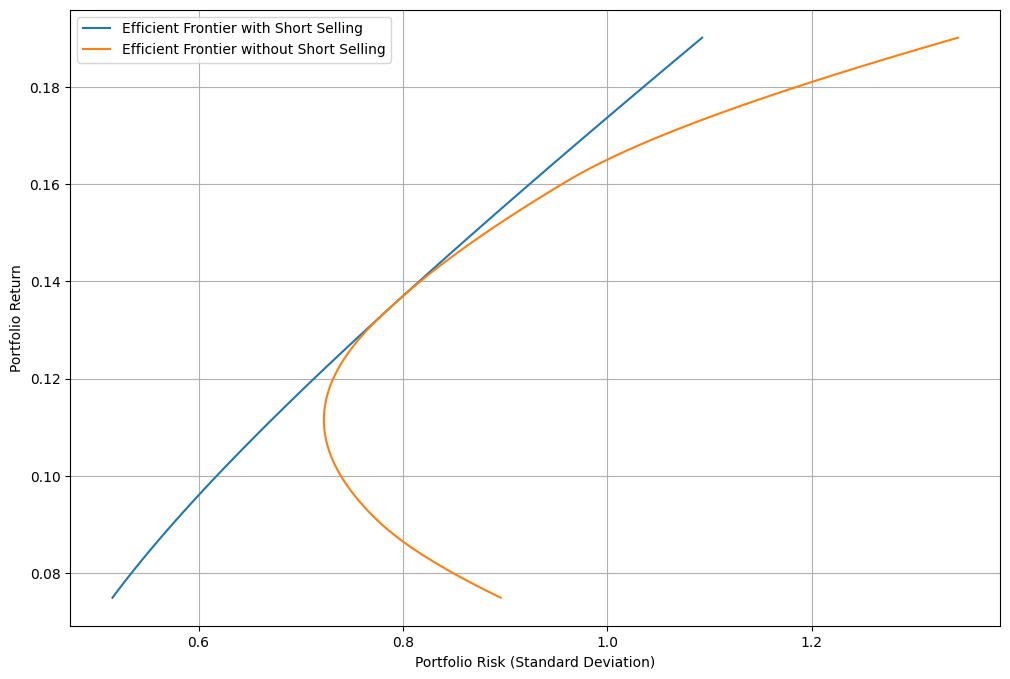
\includegraphics[width=\linewidth]{assets/efficient-frontier-comparison.png}
    \caption{Comparison of efficient frontiers with and without short selling constraint}
    \label{fig:efficient-frontier-comparison}
\end{figure}

As it can be clearly seen, for a given risk level the optimal portfolio without the short selling constraint has expected returns equal or greater than the optimal portfolio with the constraint. 

Any strategy that allows for both the buying and selling of assets is called a long-short trading strategy, and there are many such strategies with different purposes and characteristics. The strategy that will be studied in this work belongs to a type of long-short strategies called pairs-trading strategies.

\subsubsection{Pairs-trading strategies}
These strategies were first developed by a group of traders at Morgan Stanley in 1985 under the leadership of Nunzio Tartaglia (\cite{pole_2011}) and they follow a very simple principle. There are sometimes pairs of assets that move very similarly, like the case of Aveco Biotechnology and Dover Corporation, whose prices are shown in \autoref{fig:cointegrated-assets}.

\begin{figure}[h]
    \captionsetup{justification=centering}
    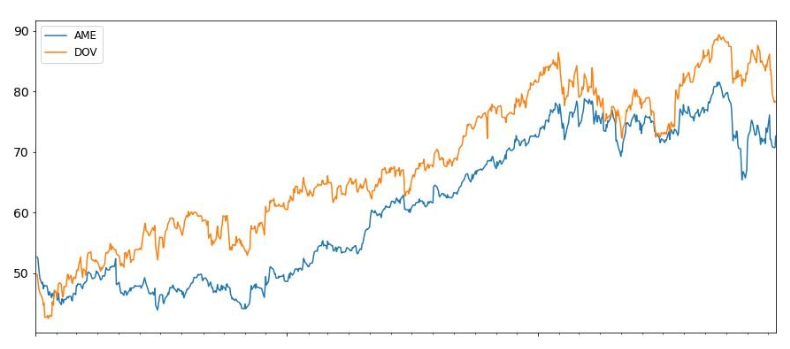
\includegraphics[width=\linewidth]{assets/cointegrated-assets.png}
    \caption{Stock prices of two cointegrated assets. Source: \href{https://hudsonthames.org/definitive-guide-to-pairs-trading/}{Hudson and Thames: The comprehensive introduction to pairs trading}}
    \label{fig:cointegrated-assets}
\end{figure}

If one thinks for some reason that one of the two assets is going to outperform the other, then a long position is entered in that one and a short position is entered in the other one. That way, the general movement of the market can be taken out of the position, and the profit of the trade will only depend on the difference in movement between the two assets, and not on the market movements affecting both assets. 
This can be seen more clearly with a small extension to the $CAPM$ model, where asset specific component for the returns are included.
\begin{equation}
    r_a=r_f+\beta_a(r_M-r_f)+ r_a^s+ \epsilon_a
\end{equation}
\begin{equation}
    r_b=r_f+\beta_b(r_M-r_f)+ r_b^s+ \epsilon_b
\end{equation}

A position can be chosen for both assets with position sizes $\Delta_a$ and $-\Delta_b$ and $\Delta_a\beta_a=\Delta_b\beta_b$ so that
\begin{equation}
    \label{e:market-disappears}
    r_p=\Delta_ar_a-\Delta_br_b=(\Delta_a-\Delta_b)r_f + \Delta_a r_a^s - \Delta_b r_b^s + \epsilon_p
\end{equation}
where $\epsilon_p = \Delta_a \epsilon_a - \Delta_b \epsilon_b$.

As it can be seen in equation \eqref{e:market-disappears}, the market or non specific part of the returns disappears. The portfolio returns end up depending mainly on the specific part of the returns of each of the assets, or more specifically, on the difference between these components. 

Having a strategy with returns independent to the performance of the market can be very attractive, as this strategy can in theory provide positive reutrns regardless of the general market behaviour and trends. Furthermore, by combining several sources of uncorrelated returns -- as none of them are correlated to the market any longer -- one can achieve a very well diversified portfolio with a great risk adjusted performance. 

The question of how one can find two such assets which "move very similarly" requires a bit more consideration. As outlined by \cite{review_statistical_arbitrage} there are many approaches studied in the litereature to finding such pairs. These include the Distance approach, Time series approach, Stochastic control approach, Copula approach, Principal Component Analysis approach, etc. The one that will be relevant here however is one method which relies on the idea of cointegration. 

Suppose there are two time series $X_1, X_2$, with order of integration $d$. That is, by differentiating the time series $d$ times the resulting time series is covariance-stationary -- its mean and autocovariance are constant through time and its variance is finite. The two time series are cointegrated if there exists a linear combination of the two through which the resulting time series has an order of integration of less than $d$. This can also be applied to groups of more than two time series.  

Note that this is similar to the removal of the market returns explained above but even more powerful. If enough cointegrated return time series are found, one could combine them having a portfolio with returns with a constant mean. If we know for a fact that our returns have a constant positive mean, we could have assured profits!

\subsection{Significance of understanding PnL drivers}
The Profit and Loss (PnL) of a trading strategy represents its net financial outcome, capturing the time series of gains or losses from all the trades executed under that strategy. However, the PnL itself is an aggregate measure that obscures the underlying factors contributing to the performance. Understanding the PnL drivers of a trading strategy is crucial for several reasons, particularly when it comes quantitative strategies with like the one studied in this work where the trading decisions cannot be intuitively understood. Identifying and understanding these drivers allows traders, portfolio managers, and risk managers to assess the effectiveness, risks, and potential of the strategy.

\subsubsection{Classes of PnL drivers}
\label{sec:classes-pnl-drivers}
PnL drivers are essentially the components that influence the profitability of a trading strategy. In the context of long-short strategies, these drivers can include:
\begin{itemize}
    \item \textbf{Market Exposure (Beta)}: The extent to which the strategy is exposed to broader market movements. Even in market-neutral strategies like pairs trading, unintentional beta exposure can impact PnL, especially in volatile market conditions. \cite{sharpe_1964}
    \item \textbf{Factor Sensitivities}: These refer to the strategy's exposure to various risk factors such as size, value, momentum, and volatility. For instance, a strategy with significant unintentional exposure to the momentum factor may perform well in trending markets but suffer during mean reverting market periods. \cite{asness_moskowitz_lasse_pedersen_2013}
    \item \textbf{Alpha Generation}: Alpha represents the excess return of the strategy over a benchmark or risk-free rate, and it is often seen as a key driver of PnL in active strategies. Identifying sources of alpha -- whether from market inefficiencies, behavioral biases, or other anomalies -- is central to understanding a strategy's potential for sustainable returns. \cite{feibel_2003}
    \item \textbf{Transaction Costs and Slippage}: These operational factors can erode PnL, particularly in high-frequency trading or strategies with low holding periods. Understanding how transaction costs impact net returns is vital for accurate performance measurement and optimization. \cite{gerhold_guasoni_muhle_2013}
    \item \textbf{Liquidity and Market Impact}: The liquidity of assets in the trading universe and the strategy's own impact on market prices can also be significant PnL drivers. Strategies that depend on trading less liquid instruments may encounter significant market impact, affecting overall profitability. \cite{tarun_chordia_roll_avanidhar_subrahmanyam_2001}.
\end{itemize}

\subsubsection{Importance of understanding PnL drivers}
Understanding each and all of the different drivers of a given strategy has some very relevant advantages:
\begin{itemize}
    \item \textbf{Performance Attribution and Enhancement}: By decomposing PnL into its drivers, traders can pinpoint which elements of their strategy are contributing positively or negatively to performance. This allows for targeted improvements, whether through refining factor exposures, reducing costs, or enhancing alpha generation. \cite{grinold_kahn_1999}
    \item \textbf{Risk Management}: Knowledge of PnL drivers facilitates better risk management by highlighting potential sources of risk that may not be evident from aggregate performance metrics. For example, excessive exposure to a particular risk factor can lead to significant losses if market conditions shift. \cite{ang_2014}
    \item \textbf{Strategic Adjustment and Adaptation}: Markets are dynamic, and the efficacy of a trading strategy can evolve over time. For example, historically value companies have outperfomed growth companies, but in some of the recent years this trend has reversed. A strategy that derived its performance from exposure to this factor would be affected. Understanding the underlying PnL drivers allows traders to adjust their strategies in response to changing market conditions or factor dynamics, thus maintaining or improving performance over time. \cite{lo_2004}
    \item \textbf{Investor Communication and Transparency}: For portfolio managers, clearly articulating the drivers of PnL is essential for building and maintaining investor trust. Investors are increasingly demanding transparency and want to understand the sources of returns and the risks involved in the strategies they are investing in. \cite{elif_baykal_2019}
\end{itemize}
\subsection{Factor models}
The key tool to understanding these key drivers will be factor models. Since the classical asset pricing model proposed by \cite{sharpe_1964} and \cite{lintner_1975}, many academics and practitioners have expanded and relied on factor models to describe and model asset returns. The idea behind them are quite straightforward. There exist a series of factors -- which are external known variables -- which can be used to model the returns of different assets. Each of the assets has different exposures to each of the factors, which lead to the different returns for the different assets. The general formula for factor models is thus
\begin{equation}
    r_k = \alpha_k + \sum_{i}\beta_i^k f_i + \epsilon_k
\end{equation}
where $\beta_i^k$ are the different factor loadings for asset $k$ corresponding to each of the factors $f_i$. 
Note how the classical $CAPM$ model is one such model with only one factor, the excess market returns. 
\begin{equation}
    r_a=r_f+\beta_a(r_M-r_f) + \epsilon_a    
\end{equation}

The same models that work for explaining past returns can also be used for modeling expected returns, when all the factors are stated in expected terms such as
\begin{equation}
    E\left[r_a\right]=r_f+\beta_a(E\left[r_M\right]-r_f)
\end{equation}

Another classical factor model is the one introduced by \cite{french_1992}, where two additional factors are added to compensate for the fact that there is some information regarding stock returns that isn't captured in the exposure to the market excess returns. For example, historically value stocks have outperformed growth stocks while the smaller companies within the S\&P500 have outperformed the bigger ones.
\begin{equation}
    r_a=r_f + \beta_{r_M-r_f}(r_M-r_f) + \beta_{HML}HML + \beta_{SMB}SMB + \epsilon_a
\end{equation}

These factors will be explained in more depth when the factor model used in this work is presented. 

Since the appearence of these two factor models, a huge compendium of different factors have appeared and proven with different levels of success to be determinant to stock returns. It makes no sense to review here all of these factors. However, a brief overview of the differnt types of factors can be seen in \cite{connor_1995}.
\begin{itemize}
    \item \textbf{Macroeconomic factors}: These factors are observable economic time series relating to the general economy. Some examples of such factors are the inflation rate, excess returns of long-term government bonds, percentage change in industrial production, etc. 
    \item \textbf{Fundamental factors}: These factors are characteristics of each of the stocks which have been shown to have predictive power over the returns of said stock. Some examples are firm size, BTM ratio, dividiend yield, etc. 
    \item \textbf{Statistical factors}: These factors use different statistical methods such as Maximum Likelihood Estimation or Principal Component Analysis on cross sections of asset returns to try to extract some underlying factors to all returns. 
\end{itemize}
Even though these may seem like different types of the same thing, in reality there is a crucial difference between Macroeconomic and Statistical factors and Fundamental factors. In the first two, the factors -- common to all stocks -- are observed exogenously, and then the factor loadings are obtained through a time series regression. For Fundamental factors however the process is the opposite. The betas are the ones exogenously derived, while the factor returns have to be obtained from the betas and the asset returns through a cross-sectional regression, as these factor returns cannot be observed anywhere. 
%\subsection{Literature review}
%\textcolor{green}{IS THIS REALLY NECESSARY?}
%Main long-short papers, factor models, factors influencing PnL, identify gaps
\subsection{Objectives and scope of study}
Once the basic building blocks of the study have been layed down, it is possible to explain what the purpose of the study is. 

First, a pairs-trading implementation proposed by \cite{gallego_2023} is reviewed and adapted, from a fundamental point of view to add some changes to the way the strategy proposed by \cite{ioannis_2023} was implemented and from a technical point of view, so it is able to successfully perform a backtest on a much larger universe of assets. Then, this strategy is run on an extended universe of assets and its performance is analyzed by its own merit and in comparison to a benchmark strategy. The performance is then dissected into the long and short positions sepparately and each leg is further analyzed. 
Then, a primary factor model is implemented and the returns of the strategy are analyzed through this model.  
Lastly, the alpha obtained by the strategy according to said model is further analyzed through a secondary fundamental factor model in order to further extract all possible key drivers of the returns of the strategy. 

Out of all the types of PnL drivers outlined in section \nameref{sec:classes-pnl-drivers}, only market exposure, some factor sensitivities and alpha generation are analyzed. Transaction costs are considered negligible due to the daily frequency of transactions and the small impact compared with the other factors, while slippage and liquidity and market impact have also been ignored due to the high trading volume of the selected universe of assets, the S\&P500. 

\newpage
\section{Methodology}
After having introduced the main concepts needed to understand the outline and progression of this work, it is possible now to enter the specifics of the work carried out. In this section, the specific pairs-trading strategy will be outlined, together with the benchmark pairs trading strategy used as comparison and the two factor models used to understand its PnL drivers.
\subsection{Strategy description}
The strategy selected to be analyzed has been the one introduced by \cite{ioannis_2023}. In their paper they outline a statistical arbitrage pairs trading strategy based on a two agent framework. 

One agent, the investor, has a cointegration model that indicates when in a pair one of the assets is relatively overvalued and the other is relatively undervalued. These mispricings are mean reverting, and the investor can profit from them by shorting the overvalued asset and buying the undervalued one. The other agent, the counter-party, receives the order flow from the investor taking the opposing position and is required by  operational mandate to continuously hedge the position and neutralize the portfolio. Within this framework, by maximizing the expected utility of the portfolio, the optimal weights for the investor are shown to be the deltas of a spread option on the two assets. 

The basic cointegration model used by the investor of two assets with prices $y_t$ and $x_t$ is 
\begin{equation}
    \frac{dy_t}{y_t}=\mu_ydt-\lambda_1z_tdt+\sigma_ydW_{y,t}
\end{equation}
\begin{equation}
    \frac{dx_t}{x_t}=\mu_xdt+\lambda_2z_tdt+\sigma_xdW_{x,t}
\end{equation}
\begin{equation}
    z_t=\ln y_t - \ln x_t
\end{equation}

where $\mu_y$, $\mu_x$, $\lambda_1$, $\lambda_2$, $\sigma_y$ and $\sigma_x$ are constant parameters and $W_{y,t}$ and $W_{x,t}$ are standard Brownian motions with zero drift rate and unit variance rate. Additionally, the investor has a cash account $B_t$
with a constant return $r$ following the dynamics
\begin{equation}
    dB_t=rB_tdt
\end{equation}
With that, the investor's portfolio is the following.
\begin{equation}
    \label{e:portfolio-equation}
    \Pi_t=\delta_1 y_t + \delta_2 x_t + \delta_3 B_t
\end{equation}
Where $\delta_1$, $\delta_2$ and $\delta_3$ are the position sizes for the two assets and the cash account respectively. This portfolio equation is subject to the constraint 
\begin{equation}
    \delta_1 + \delta_2 + \delta_3 = 1
\end{equation}
ensuring the portfolio position is self financed between the long, short and cash positions. 

Having the two cointegrated assets, a call option written on the spread $y_t - x_t$ with payoff $\psi(y_T, x_T)=max(y_T-x_T,0)$ can be defined as 
\begin{equation}
    C(y_t,x_t,t)=y_t \Phi(d_1)-x_t \Phi(d_2)
    \label{spread_option}
\end{equation}
where:
\begin{equation}
    \label{e:calc-d1}
    d_1=\frac{\ln\left(\frac{y_t}{x_t}\right)+\frac{1}{2}\sigma^2_z(T-t)}{\sigma_z \sqrt{T-t}}
\end{equation}
\begin{equation}
    d_2=d_1-\sigma_z \sqrt{T-t}
\end{equation}
\begin{equation}
    \sigma_z=\sqrt{\sigma_y^2+ \sigma_x^2-2\rho_{yx}\sigma_y\sigma_x}
\end{equation}
Given that option, in order to hedge the option position the counter-party must hold $\Delta_t$ shares of the underlying asset at time t. The two different $\Delta_t$ for the spread option are given by 
\begin{equation}
    \label{e:position-size-model-1}
    \Delta_{y,t} = \frac{\partial C}{\partial y} = \Phi(d_1)+\left[\phi(d_1)-\frac{x_t}{y_t}\phi(d_2)\right] \frac{1}{\sigma_z \sqrt{T-t}}=\Phi(d_1)
\end{equation}
\begin{equation}
    \label{e:position-size-model-2}
    \Delta_{x,t} = \frac{\partial C}{\partial x} = -\Phi(d_2)-\frac{y_t}{x_t}\left[\phi(d_1)-\frac{x_t}{y_t}\phi(d_2)\right] \frac{1}{\sigma_z \sqrt{T-t}}=-\Phi(d_2)
\end{equation}
The optimal position sizes for the investor are demonstrated to be equivalent to the postions yielded by the hedging strategy of the counter-party:
\begin{equation}
    \label{e:position-sizes}
    \varphi^*_1=\Delta_y,\quad \varphi^*_2=\Delta_x
\end{equation}
Through this equivalence, an optimal trigger for the investor to  enter and exit the position is determined. The investor must buy asset $y$ and short asset $x$ whenever 
\begin{equation}
    \label{e:trigger-1}
    \ln\left(\frac{y_t}{x_t}\right) > (1-\lambda_1 - \lambda_2)\sigma_z
\end{equation}
and conversely he must buy asset $x$ and short asset $y$ when
\begin{equation}
    \ln\left(\frac{x_t}{y_t}\right) > (1-\lambda_1 - \lambda_2)\sigma_z
\end{equation}
By using implied volatilities obtained from the option markets of each of the assets, this trigger is forward looking and thus should be more accurate than other usual triggers relying on historical volatility values. 

Furthermore, this dynamic trigger is more precise and adjustable than others relying on fixed values e.g. enter the position when the spread is over 2 standard deviations of the historical spread.

\subsection{Benchmark description}
For the benchmark to be significant, it also has to be a pairs-trading, mean-reverting, market-neutral benchmark. Only by comparing the strategy to such a benchmark strategy can its true successes come to light. In order to fulfill all the mentioned criteria, the following pairs-trading strategy has been chosen as the benchmark. 

The first step for implementation of this strategy is to test for cointegration for all asset pairs through the Johansen test as proposed by \cite{johansen_1991}. 
For this test, suppose we have a vector of two time series of logprices  $X_t=[X_{1t},X_{2t}]'$. 
Consider a general $VAR$ model of order $k$ written in the error correction form 
\begin{equation}
    \Delta X_t = \mu + \sum_{i=1}^{k-1}{\Gamma_i \Delta X_t-i} + \Pi X_{t-k} + \Phi D_t + \epsilon_t
\end{equation}
where $\mu$ is the drift component of the series, $\Pi$ is the $p\times p$ matrix determining long-run relationships between variables, $\Gamma_i$ are short-run coefficient matrices, $\Phi D_t$ is a seasonal adjustment term and $\epsilon_t$ is a Gaussian error term. In the specific implementation used for the benchmark, it is assumed $\Phi D_t=0$ as the logprice series have no seasonal components, and the order of the model is $k=1$. 
The matrix $\Pi$ Can be further broken down as 
\begin{equation}
    \Pi=\alpha \beta '
\end{equation}
where $\beta$, the cointegration vectors and $\alpha$, the adjustment coefficients determining the speed of return to equilibrium, are $p\times r$ matrices. 
The Johansen test has two variations, the eignevalue test and the trace test -- being the latter one the one which was used in this implementation. In the trace test, the null hypothesis tests for the rank of the $\Pi$ matrix through
\begin{equation}
    H_0: r \leq r_0
\end{equation}
Finally, the resulting $r$ is taken as the number of cointegrated relationships. In this case with only two assets, there is at most $r=1$ cointegrated relationship and thus a single hypothesis test needs to be performed. 

Once all pairs have been tested for cointegration, for the next time period those cointegrated pairs are considered for trading. According to the tested relationship, the portfolio logprice $X_p$ should be stationary, where
\begin{equation}
    X_p = \lambda_1 X_1 + \lambda_2 X_2
\end{equation}
with $\lambda_1$ and $\lambda_2$ being the two components of the eigenvector corresponding to the maximum eigenvalue obtained in the Johansen test.

The historical mean and standard deviation of that combined logprice is calculated, and the position is entered when the combined logprice deviates more than two standard deviations from the mean. 
\begin{equation}
    \mu_{X_p} - 2\sigma_{X_p} \geq X_{p,t} \quad \text{or} \quad X_{p,t} \geq \mu_{X_p} + 2\sigma_{X_p}
\end{equation}
The sense of the position -- which asset to go long and which to go short -- depends on whether the two standard deviation barrier is exceeded above or below the mean.

When that trigger is activated, the position is entered ensuring the ratio of position sizes between both assets is equivalent to the ratio of values in the mentioned eigenvector. The portfolio is rebalanced daily to maintain that ratio \cite{chan_2013}.
Once the combined logprice crosses the historical mean, the position is closed. 

\subsection{Primary factor model description}
As the primary tool for analyzing the PnL drivers of the strategy's profits, an extension of the four factor model proposed by \cite{carhart_1997} has been used. To these four factors, the Idiosyncratic Volatility Spread ($IVS$) addressed in \cite{ioannis_2024} has been added as a potential driver of profit for the strategy. The model thus becomes
\begin{multline}
    \label{e:primary-regression}
    r_s = \alpha^{(1)} + \beta_{r_M-r-f}(r_M-r_f) + \beta_{HML}HML + \beta_{SMB}SMB + \\ + \beta_{MOM}MOM+ \gamma_{IVS}IVS + \epsilon^{(1)}
\end{multline}

The factors present in the model are the following 
\begin{itemize}
    \item $r_M-r_f$: The market risk premium is a factor that represents the excess returns of the market -- in this case the S\&P500 -- over the risk free rate, taken from the 6 month Treasury Bill. 
    \item $HML$: High-minus-low, or value premium is a factor representing the spread in returns between the value stocks and the growth stocks. Here, value stocks are those with the highest Book-to-Market ratio and growth stocks are those with the lowest BTM ratio.
    \item $SMB$: Small-minus-big or size premium is a factor representing the spread in returns between the small companies and the big companies. That is, those with the lowest and highest market capitalization respectively.
    \item $MOM$: Up-minus-down or momentum is a factor representing the spread in returns between companies that performed the best in the last 12 months and the companies that performed the worst in that same recent period. 
    \item $IVS$: The Idiosyncratic Volatility Spread is a factor representing the spread in volatility between the given stock and the market. Note how this is the first fundamental factor out of all of the rest.
\end{itemize}

The $\alpha^{(1)}$ is the outperformance -- or underperfomance -- of the strategy with respect to the model that cannot be explained solely by these five factors. 

To obtain the given regression, the daily returns of the strategy are regressed in a panel regression for each stock, where the macroeconomic factors are common to all assets and the $IVS$ is particular to each one. 

Other factors were considered for the regression. Mainly, these are the individual stock's volatility premium and the overal S\&P500's volatility premium. That is, the spread between the rolling 1 month historical volatility and the implied volatility. A visualization of this spread for the S\&P500 can be seen in \autoref{fig:hist-vs-impl-vol}. However when these variables were introduced in the regression problems of multicollinearity arose, due to their similarity to the $IVS$, leading to instability in the estimation of the regression coefficients and clouded results in the t-test for each of the individual coefficients. To solve these problems, these variables had to be dropped leaving the five factor model explained above.

\begin{figure}[ht]
    \captionsetup{justification=centering}
    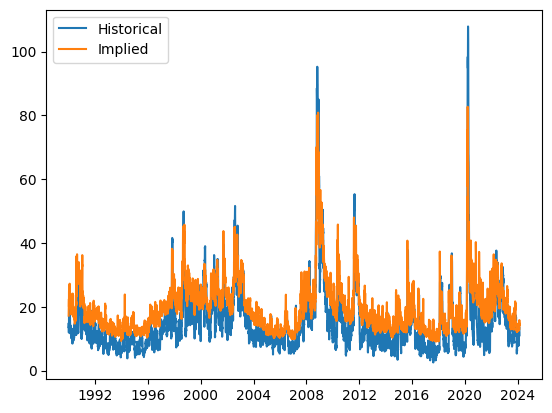
\includegraphics[width=\linewidth]{assets/hist-vs-impl-vol.png}
    \caption{Comparison of historical rolling 1 month volatility and implied 1 month volatility for the S\&P500}
    \label{fig:hist-vs-impl-vol}
\end{figure}

\subsection{Secondary factor model description}
As outlined by \cite{fama_french_1995}, there are other fundamental factors that affect the returns of stocks and of trading strategies. Many of the fundamental factors however, like the Book-to-Market outlined in this paper and others, are only observable as quarterly data in the best case, while all previous factors were observable daily. In order to run the previous factor analysis with as much data density as possible, but also to understand how these other factors affect the strategy's performance, a secondary regression has been created. 

The already presented primary regression is performed on a rolling basis. For every quarter, the primary regression is run and the $\alpha$ of said regression is kept so as to obtain a series of quarterly $\alpha$. These $\alpha$ are then regressed on these new quarterly factors, shedding some light into the drivers of the excess returns found with the first regression. This secondary model is the following.
\begin{multline}
    \label{eq:secondary-regression}
    \alpha^{(1)}=\alpha^{(2)} + \gamma_{MKTVal}MKTVal + \gamma_{BTM}BTM + \gamma_{PER}PER + \gamma_{EVEBIT}EVEBIT + \\ + \gamma_{EVEBITDA}EVEBITDA + \gamma_{GPA}GPA + \gamma_{ROC}ROC + \epsilon^{(2)}
\end{multline}
These factors have been shown to be drivers of portfolio performance in \cite{ramon_bermejo_climent_2021}. The meaning behind those factors is the following
\begin{itemize}
    \item $MKTVal$: The market value of the stock, measured in market capitalization.
    \item $BTM$: The Book-to-Market ratio of the stock.
    \item $PER$: The Price-to-Earnings ratio of the stock.
    \item $EVEBIT$: The Enterprise Value to EBIT ratio of the stock. 
    \item $EVEBITDA$: The Enterprise Value to EBITDA ratio of the stock.
    \item $GPA$: The Gross Profits to Assets ratio of the stock.
    \item $ROC$: The Return on Capital ratio of the stock. 
\end{itemize}
The first 5 regressors are a proxy for the value characteristic of the stock, while the last 2 showcase the profitability characteristic of the stock. 

In a similar way to the last regression, the resampled alpha is regressed in a panel regression over all stocks for all time periods, where each of these factors -- all fundamental -- are unique for each stock. The main difference in how this regression was conducted as oposed to the last one is in the preprocessing of the factors. In this regression, there are some very significant defferences in the order of magnitude of the factors, with some being ratios in the unit scale and others -- namely the Market Value -- being in the order of the billions. In order to avoid numerical problems during the estimation of the coefficients, all factors have been scaled through min-max scaling.
\newpage
\section{Data Description}
\label{sec:data-description}
Throughout the analysis conducted in this work, several different data sources have been used:
\begin{itemize}
    \item Asset prices: In order to retrieve the daily asset prices for the components of the S\&P500, the FactSet API was used. The closing price of the session was taken as the daily price. The time period for the data encompassed from the ending of 2005 to the beginning of 2024, and all companies that formed part of the S\&P500 for the whole period were considered. 
    \item Implied volatilities: Another key component of the strategy's trigger and sizing are the volatilities implied by the 1 month options. These volatilities were also obtained from the FactSet API. 
    \item Risk free rate: The Risk free rate, another key component for several of the calculations used in the strategy, was taken as the 6 month US Treasury Bill rate. These rates were obtained directly from the US Federal Reserve System.
    \item Factors: The different factors were obtained from different sources
    \begin{itemize}
        \item $r_M-r_f$: The market excess returns were constructed from the returns of the S\&P500 obtained from the aforementioned dataset, subtracting the already obtained risk free rate.
        \item Macroeconomic factors: The daily $SMB$, $HML$ and $MOM$ factors were obtained from the Kenneth R. French online Data Library, hosted by Dartmouth College.
        \item $IEP$: The Idiosyncratic Equity Volatility Premium was calculated taking the rolling historical 1 month volatility of the stocks, calculated from the already obtained daily price data, and subtracting the 1 month historical volatility of the S\&P daily price. This measure is then turned into daily volatility values for each stock. For a more in depth descussion about the Idiosyncratic Equity Volatility Premium refer to \cite{ioannis_2024}.
        \item Other Fundamental Factors: The rest of the fundamental factors, corresponding to disclosed financial data from the companies, are obtained from the FactSet API. 
    \end{itemize}
\end{itemize}
\newpage
\section{Technical Description}
As a starting point for the implementation, the work by \cite{gallego_2023} has been kindly taken as reference. In order to better follow the changes here pointed out, it is recommended to first refer to that work.

The main changes performed on the implementation of the strategy are the following:

\begin{itemize}
    \item \textbf{Position sizing}: In the original work, once the trigger was activated, the positions were opened with the position size determined on the day of the trigger change. That position was then kept until the position was determined to be closed. In the new position sizing, the position is also entered on the moment the trigger is activated but it is changed daily in accordance with the daily changes in position sizes as calculated in equation \eqref{e:position-sizes}. This allows for, on the one hand, better performance as the dynamic position sizing better follows the specification of the position sizing model in equations \eqref{e:position-size-model-1} and \eqref{e:position-size-model-2}, better adjusting to changes in implied volatilty and price changes. On the other hand, this also allows for calculating the position sizes in a vectorized way from the trigger vector, making the position sizing calculation process faster and more efficient. 
    \item \textbf{Return calculation}: In the original implementation, returns for each timestep were calculated as a sum of the returns of the long and short positions. This was changed to consider the full portfolio equation \eqref{e:portfolio-equation} taking into account the returns of the cash position -- positive or negative -- as the long and short positions are hardly ever completely self financed. The return calculation function was also extended in order to extract the long and short returns separately from the overall returns. 
    \item \textbf{Spread option $\Delta$}: The calculation of the $d_1$ as per \eqref{e:calc-d1} was modified in order to remove the risk free rate from the numerator and to remove an absolute value on the difference between logprices. 
    \item \textbf{Trigger}: The trading trigger was modified to fit exactly equation \eqref{e:trigger-1}. This was also a simpler and faster implementation than the previous trigger. 
    \item \textbf{Win rate}: An in-built counter has been implemented to measure what percentage of the positions end up yielding returns higher than the risk free rate for the period in which they are traded. This win rate is calculated for overall returns, long returns and short returns. 
    \item \textbf{Active positions}: Similarly to the win rate, an in-built counter has been implemented to measure the number of pairs which are being actively traded on any given day.  
    \item \textbf{Pairs considered}: Since the cointegration estimator and the position sizing methods assumes which asset of the pair is long and which is short, the set of pairs considered for trading has been extended to enable both assets to be either long or short in all pairs. 
    \item \textbf{Process batching}: In order to enable the strategy to be run on a much larger universe of assets, the parameter estimation process and the return calculation process for all pairs has been divided into batches. After a given batch of pair's parameters are estimated, they are saved as a pickle file. The joint returns of that set of pairs are calculated and again saved to permanent memory as a pickle file, only after the returns of pairs in which the trigger was not activated for the whole period are erased to reduce the unnecessary use of memory. The variables containing all pair parameters and return calculations are erased from RAM and the next batch of pairs can be calculated. If the process crashes, it does not have to restart from the beginning as the batches which have already finished have been saved and don't need to be calculated again. 
    \\After all batches have been calculated, all saved sets of returns are read into memory and aggreagated, yielding the final set of strategy returns, which can be then finally saved for later analysis. This batching process had to be implemented as the CPU did not have enough memory to hold all the variables for the parameter estimation process or the return calculation process for all pairs, even though most of the calculations were already performed in parallel in the original implementation and thus the variables were reused reducing the memory footprint. The memory profiling of the program before the changes were implemented can be seen in \autoref{fig:memory-profile}.
    \newpage
    \begin{figure}[h]
        \centering
        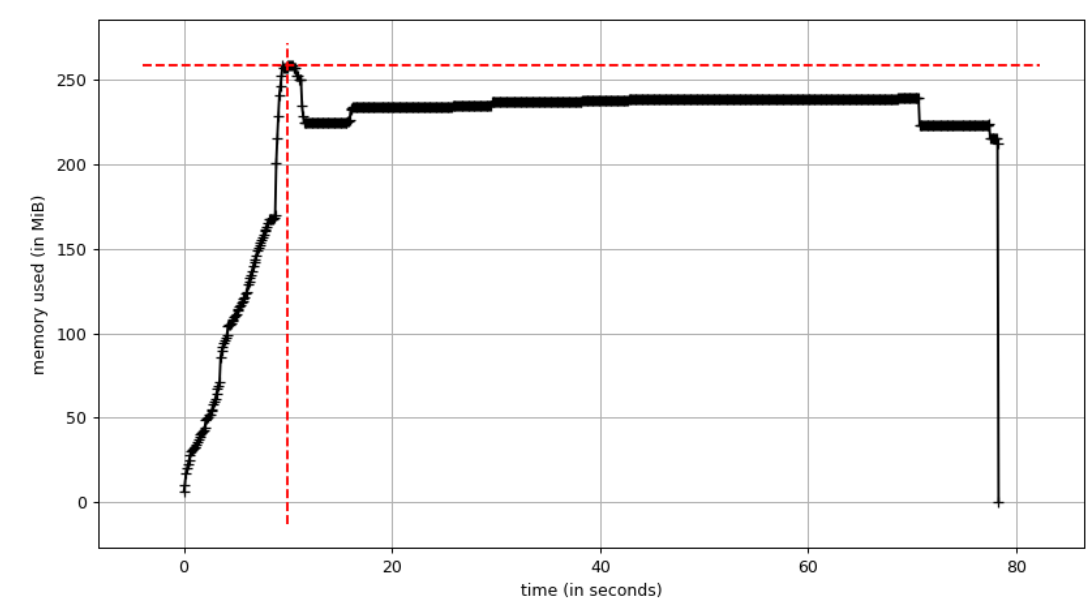
\includegraphics[width=300px]{assets/memory-profile.png}
        \caption{Memory profile of execution before introduction of batching}
        \label{fig:memory-profile}
    \end{figure}
    
    In the figure it can be seen how the memory usage grows fast in the parameter estimation process, and after a peak is reached, the process tries to maintain the execution running bu is finally killed after about a minute. 
\end{itemize}
\newpage
\section{Results}
In this section, the main results of the analysis will be shown. Given the twofold goal of this work, two sections will be needed. One for the performance of the strategy and one analyzing the PnL drivers of said performance. 

\subsection{Strategy}
In this section, the performance of the strategy will be shown. First, it will be presented in comparison to the overall market, then as a comparison to the calculated benchmark and finally disaggregating the long and short legs of the strategy. 

\subsubsection{Overall Performance}
\label{sec:overall-performance}
In order to showcase the performance of the newly implemented strategy, several visual representations and usual metrics for measuring performance and risk will be shown in comparison with the S\&P500 as a very basic reference point. 

\begin{figure}[ht]
    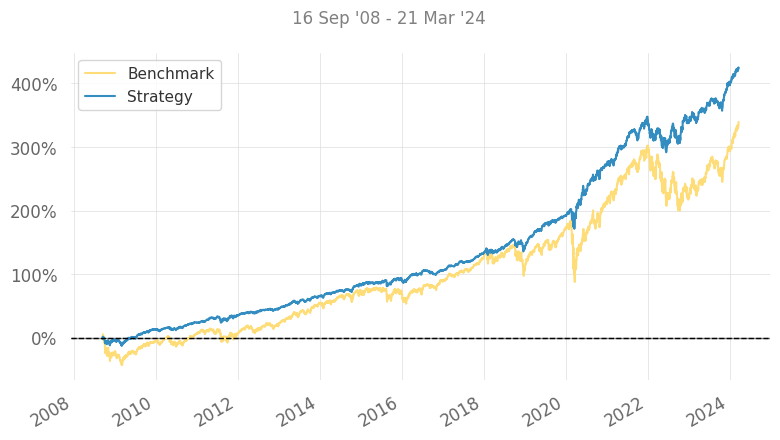
\includegraphics[width=\linewidth]{assets/strat-vs-sp500.png}
    \caption{Cumulative returns of the strategy compared with the S\&P500}
    \label{fig:strat-vs-sp500}
\end{figure}

The most basic way in which one can start to see the performance of the trading strategy is looking at how the cumulative returns evolve over time compared with the S\&P500. In \autoref{fig:strat-vs-sp500} it can be seen how the overall cumulative returns are higher, and seemingly less volatile. 
In order to understand whether the volatility truly is lower, a useful visualization is the volatility-matched returns of the strategy.

\begin{figure}[ht]
    \captionsetup{justification=centering}
    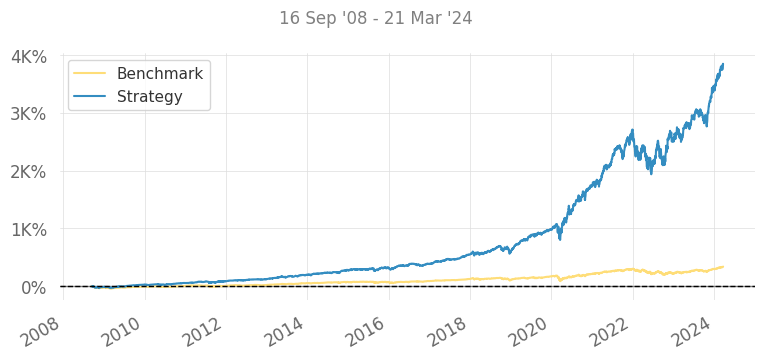
\includegraphics[width=\linewidth]{assets/strat-vs-sp500-vol-matched.png}
    \caption{Cumulative returns of the volatility matched strategy compared with the S\&P500}
    \label{fig:strat-vs-sp500-vol-matched}
\end{figure}
These are the returns that would be obtained investing in the strategy if the position were leveraged enough to match the volatility of the S\&P500. That is, if the investor were to borrow enough money and put it in the strategy so that the volatility of said setup is the same volatility as the benchmark. The returns are thus:
\begin{equation}
    r_{vm}=\frac{\sigma_b}{\sigma_s}r_s
\end{equation}
where $r_{vm}$ are the volatility matched returns, $\sigma_b$ is the benchmark's volatility, $\sigma_s$ is the strategy's volatility and $r_s$ is the strategy's returns. 
If a given investor is comfortable enough with the level of risk given by a basic market investment, these are the equivalent results that could be obtained with the given strategy.

Appart from visualizing the cumulative performance, it will also be helpful to showcase some numerical results. 

\begin{table}[ht]
    \centering
    \begin{tabular}{rll}
        \toprule
        Metric & \multicolumn{2}{c}{Value} \\ 
        \cmidrule(lr){2-3}
            & Strategy & S\&P500 \\
        \midrule
        CAGR & 7.65\% & 6.81\% \\
        Annualized Volatility & 8.79\% & 20.45\% \\
        Skew & 0.14 & -0.29 \\
        Kurtosis & 7.9 & 12.65 \\
        \bottomrule
    \end{tabular}
    \caption{Main moments of the strategy's return distribution}
    \label{table:main-moments-strat-vs-sp500}
\end{table}

As a sidenote, it can be seen how the CAGR for the S\&P500 is much lower than the mean annual returns that have been recorded during this period. That is because the CAGR takes into account how the price movements compound over time, and thus volatility, skewness and kurtosis effects are also present. The mean compounded returns are thus not $r_c=\mu$, but 
\begin{equation}
    r_c=\mu-\frac{1}{2}\sigma^2+\frac{1}{3}S\sigma^3-\frac{1}{4}K\sigma^4  + \mathcal{O}\left(\sigma^5\right)
\end{equation}
where $\mu$ are the mean annual returns, $\sigma$ is the annualized standard deviation of the returns, $S$ is the skewness and $K$ is the kurtosis of the return distribution. This is thus a more representative figure of the expected long term returns than if mean annual returns were showcased here.

In \autoref{table:main-moments-strat-vs-sp500} four metrics referring to the four first moments of the return distributions can be seen. 
It confirms numerically what was already intuited by watching the cumulative distribution of \autoref{fig:strat-vs-sp500}, returns are higher on average and risk -- as measured by the volatility -- is lower. However, by looking at the next two moments more interesting information is uncovered. While stock returns are well known to generally exhibit a negative skew as shown in \cite{peiro_1999} and confirmed here with the S\&P500 returns, the strategy manages to obtain positive skew returns. Similarly for kurtosis, even though the strategy's value still lies above the normal distribution's 3, it is considerably lower than the market's kurtosis.

This can be visualized very nicely in \autoref{fig:strat-vs-sp500-ret-dist}, where the monthly return distribution for both sets of returns are shown. 

\begin{figure}[ht]
    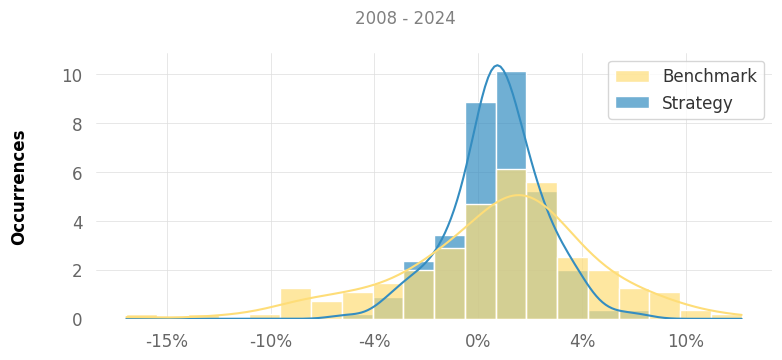
\includegraphics[width=\linewidth]{assets/strat-vs-sp500-ret-dist.png}
    \caption{Monthly returns distribution of the strategy compared with the S\&P500}
    \label{fig:strat-vs-sp500-ret-dist}
\end{figure}

Apart from the already presented metrics, which are seen clearly in the distribution plot, it can be seen how it could seem like the mean of the distribution for the S\&P500 is higher than that of the strategy. However, the only thing that is clearly higher is the mode, and the more extreme negative movements experienced by the benchmark really weigh down on the long run average compounded returns. 

Some other risk-adjusted measures for the strategy are 
\begin{table}[ht]
    \centering
    \begin{tabular}{rll}
        \toprule
        Metric & \multicolumn{2}{c}{Value} \\ 
        \cmidrule(lr){2-3}
            & Strategy & S\&P500 \\
        \midrule
        Sharpe ratio & 1.16 & 0.51 \\
        Sortino ratio & 1.69 & 0.73 \\
        Calmar ratio & 0.54 & 0.15 \\
        Max Drawdown & -14.15\% & -46.1\% \\
        Longest Drawdown & 335 & 821 \\
        Alpha & 0.12 & - \\
        Beta & -0.06 & - \\
        Correlation & -13.88\% & - \\
        Treynor ratio & -7103.63\% & - \\
        \bottomrule
    \end{tabular}
    \caption{Risk and risk-adjusted return metrics for the strategy}
    \label{table:risk-adjusted-strat-vs-sp500}
\end{table}

In \autoref{table:risk-adjusted-strat-vs-sp500} the intuition gained with the previous metrics is solidified. Through the main risk-adjusted return metrics it can be seen how the strategy's performance is clearly superior to that of the S\&P500. Regarding other purely risk measures like those relative to drawdowns, it can also be seen how the periods of losses with the strategy are less acute and shorter. Finally, it can also be seen how the strategy's performance is completely market neutral if not slightly opposite to the market, with a slightly negative beta and correlation. This means that the strategy can be effectively used as a hedge to a market investment, partially compensating in moments of low or negative market returns. The superior performance together with the hedging and diversification potential it brings provides for a very significant alpha. 

For a more in depth explanation of these metrics, how they are calculated and their general interpretation and significance refer to \autoref{sec:performance-metrics-explained} \nameref{sec:performance-metrics-explained}.

When taking a dynamic view of these figures, it can be seen how temporally robust the findings are.

\begin{figure}[ht]
    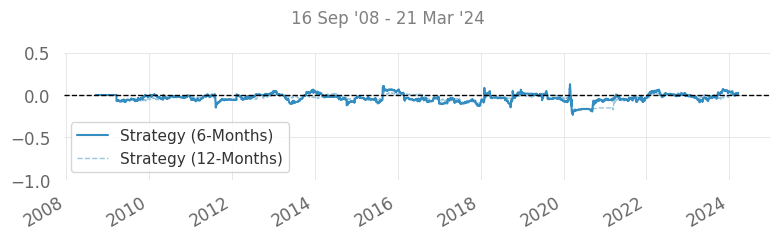
\includegraphics[width=\linewidth]{assets/strat-vs-sp500-rolling-beta.png}
    \caption{6 and 12 month rolling beta of the strategy's returns with respect to the S\&P500}
    \label{fig:strat-vs-sp500-rolling-beta}
\end{figure}

In \autoref{fig:strat-vs-sp500-rolling-beta} the rolling beta can be seen. That is, at each point in time the beta obtained with the previous 6 or 12 month window. Observing this figure it can be seen how the beta of the strategy stays consistently very close to zero and generally on the negative side, with very few ocurrences of the beta becoming positive. It is specially significant how in the moments of biggest crisis, i.e. the 2020 Covid-19 market crash, the beta becomes even more significantly negative showcasing the resilience of the strategy to market crashes. This is conforms perfectly with the results obtained by \cite{ioannis_2023}. This behaviour is specially relevant given the findings by \cite{sandoval_franca_2012} showing that during market crashes most assets become a lot more strongly correlated, making it even more difficult for investors to diversify their investments in these times. 

% Finally, some other more practical metrics that could be useful from the trading perspective
% \begin{table}[ht]
%     \centering
%     \begin{tabular}{rll}
%         \toprule
%         Metric & \multicolumn{2}{c}{Value} \\ 
%         \cmidrule(lr){2-3}
%             & Strategy & S\&P500 \\
%         \midrule
%         Sharpe ratio & 1.16 & 0.51 \\
%         Sortino ratio & 1.69 & 0.73 \\
%         Omega ratio & 0.14 & -0.29 \\
%         Max Drawdown & -14.15\% & -46.1\% \\
%         Longest Drawdown & 335 & 821 \\
%         Alpha & 0.12 & -- \\
%         Beta & -0.06 & -- \\
%         Correlation & -13.88\% & -- \\
%         Treynor ratio & -7103.63\% & -- \\
%         \bottomrule
%     \end{tabular}
%     \caption{Risk and risk-adjusted return metrics for the strategy}
%     \label{table:risk-adjusted-strat-vs-sp500}
% \end{table}

A final aspect of the performance of the strategy which has not been discussed until this point is the number of trades or assets it effectively enters positions in. This can be seen in \autoref{fig:strat-open-pairs}.

\begin{figure}[ht]
    \captionsetup{justification=centering}
    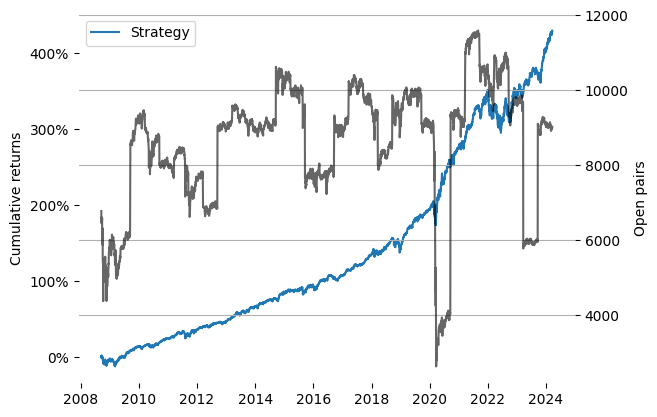
\includegraphics[width=\linewidth]{assets/strat-open-pairs.png}
    \caption{Pairs with open positions taken by the strategy together with the cumulative returns}
    \label{fig:strat-open-pairs}
\end{figure}

In \autoref{fig:strat-open-pairs} it can be seen that at any given point there are between $\sim$12.000 and $\sim$3.000 pairs being traded, with the average being around $\sim$9.000. For a position to be open in a given pair, that pair needs to have been found to be cointegrated in the previous time period, and in the current day the trading trigger needs to have been activated. In 500 stocks, the total possible number of pairs is of 124.750. However, not all 500 stocks have been members of the index for the whole time period, so only 398 stocks are effectively used, which gives a total of 79.003 potential pairs. This means, that on average the strategy is trading $\sim$11\% of all possible pairs. 

It is also relevant how there doesn't seem to be any clear relationship between the number of pairs being traded and the distribution of returns, with returns behaving similarly in periods of high volume of open positions and in periods of low volume of open positions. 

\subsubsection{Comparison with Johansen Portfolio}
After having seen in general terms what the performance of the strategy looks like, it is pertinent now to compare it with a more similar strategy, that of the Johansen cointegration portfolio. This is another pairs-trading cointegration based strategy, and thus it is expected to be a lot more similar than to the S\&P500. The general comparison of the cumulative returns of both is the following:

\begin{figure}[ht]
    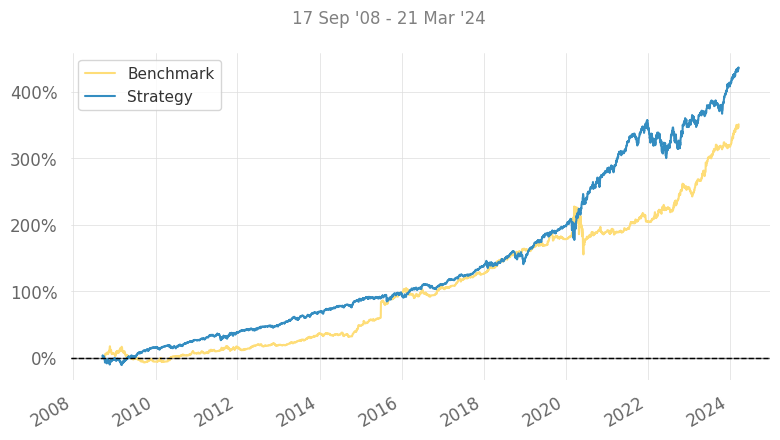
\includegraphics[width=\linewidth]{assets/strat-vs-johansen.png}
    \caption{Cumulative returns of the strategy compared with the S\&P500}
    \label{fig:strat-vs-johansen}
\end{figure}

From a first glance it can be seen how this is a much more even comparison than with the S\&P500. The performance of the Johansen portfolio exhibits higher overall cumulative returns and apparently lower volatility throughout the period. However, the overall returns of the selected strategy still lie above those of the Johansen portfolio. As for the volatility, it is hard to judge simply graphically, and thus the precise numbers are shown in \autoref{table:main-moments-strat-vs-johansen}

\begin{table}[ht]
    \centering
    \begin{tabular}{rll}
        \toprule
        Metric & \multicolumn{2}{c}{Value} \\ 
        \cmidrule(lr){2-3}
            & Strategy & Johansen \\
        \midrule
        CAGR & 7.65\% & 6.93\% \\
        Annualized Volatility & 8.79\% & 8.84\% \\
        Skew & 0.14 & 3.03 \\
        Kurtosis & 7.9 & 92.03 \\
        \bottomrule
    \end{tabular}
    \caption{Main moments of the strategy's return distribution}
    \label{table:main-moments-strat-vs-johansen}
\end{table}

It can be seen how the annual returns are ever so slightly superior for the strategy compared to the Johansen portfolio and the annualized volatility is actually lower, although marginally. However, the comparison for the skew and kurtosis should be made more carefully. If the cumulative returns graph for the Johansen portfolio in \autoref{fig:strat-vs-johansen} is inspected carefully, it becomes apparent how in 2020 -- during the midst of the Covid-19 market crash -- there is a very abrupt movement in the cumulative reutrns graph. Due to the positions taken by the Johansen strategy, there is a great profit and then loss, which accentuates the weight of the extremes and biases the kurtosis metric. The similarity between both distributions can be better seen graphically in \autoref{fig:strat-vs-johansen-ret-dist}.

\begin{figure}[ht]
    \captionsetup{justification=centering}
    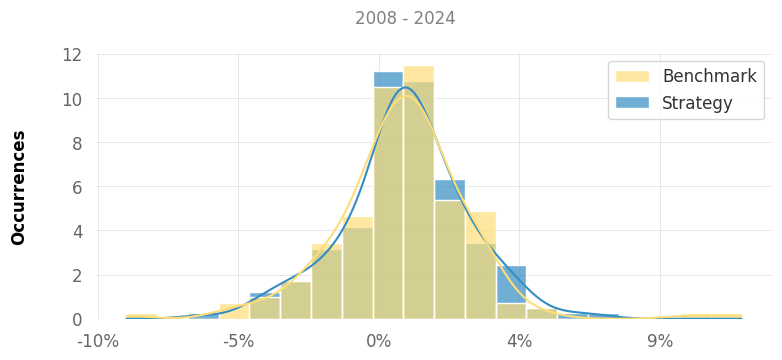
\includegraphics[width=\linewidth]{assets/strat-vs-johansen-ret-dist.png}
    \caption{Monthly returns distribution of the strategy compared with the Johansen portfolio}
    \label{fig:strat-vs-johansen-ret-dist}
\end{figure}

In \autoref{fig:strat-vs-johansen-ret-dist} it is made apparent how both distributions are much more similar than what may appear through the skew and kurtosis numbers. It can be seen in fact how the proposed pairs-trading strategy has a return distribution practically equal to its pairs-trading vanilla equivalent. It is due to high frequency of returns at around the $\sim$90\% percentile that the proposed strategy's superior performance is materialized.    

If a more practical comparison wants to be made, it could be useful to again look at the same metrics already shown in \autoref{table:risk-adjusted-strat-vs-sp500} but comparing the strategy to its new benchmark. 

\begin{table}[ht]
    \centering
    \begin{tabular}{rll}
        \toprule
        Metric & \multicolumn{2}{c}{Value} \\ 
        \cmidrule(lr){2-3}
            & Strategy & S\&P500 \\
        \midrule
        Sharpe ratio & 1.16 & 1.03 \\
        Sortino ratio & 1.69 & 1.59 \\
        Calmar ratio & 0.54 & 0.31 \\
        Max Drawdown & -14.15\% & -22.0\% \\
        Longest Drawdown & 335 & 1032 \\
        Alpha & 0.11 & -- \\
        Beta & -0.0 & -- \\
        Correlation & -0.18\% & -- \\
        \bottomrule
    \end{tabular}
    \caption{Risk and risk-adjusted return metrics for the strategy}
    \label{table:risk-adjusted-strat-vs-johansen}
\end{table}

A clear dominance by the strategy, although by margins much smaller than in the previous comparison, can be seen across all metrics. This dominance is most apparent in the drawdown statistics, where the Johansen portfolio falls prey to a long period of bad performance after the 2020 crash. The alpha of the strategy with respect to the Johansen portfolio is also apparent. And very interestingly, although both strategies are sources of uncorrelated returns, following the same principle of cointegration leveraged through pairs-trading, the correlation between both strtegies is virtually non existant. Although operating under the same principles, it seems like both strategies are able to find different pairs and take different positions throughout the whole time period. Furthermore, the pair selection method introduced in \cite{ioannis_2023} and implemented here has some advantages apart from performance related ones like finding more pairs and better performing ones. It also can be performed on a greater universe of assets in a computationally more efficient and faster way than the Johansen pair selection method. 

\subsubsection{Disaggregated Performance}
In previous sections, the general performance of the strategy as a whole has been thoroughly analyzed, against the universe of assets and against a more comparable benchmark. However, this being a pairs-trading strategy offers a possible level of analysis that hasn't been much exploited until now in the literature. It is possible to disaggregate the performance of the strategy into the long and the short leg of the strategy -- that is, the performance of all operations where the strategy went long on a stock and those where it went short on a stock -- and analyze each sepparately, observing what features of the final strategy are brought by each half. 

\subsubsubsection{Long leg}
When first looking at the long leg of the strategy's cumulative returns compared to the strategy's cumulative returns, it may seem like just by keeping the long leg better performance can be achieved.

\begin{figure}[ht]
    \captionsetup{justification=centering}
    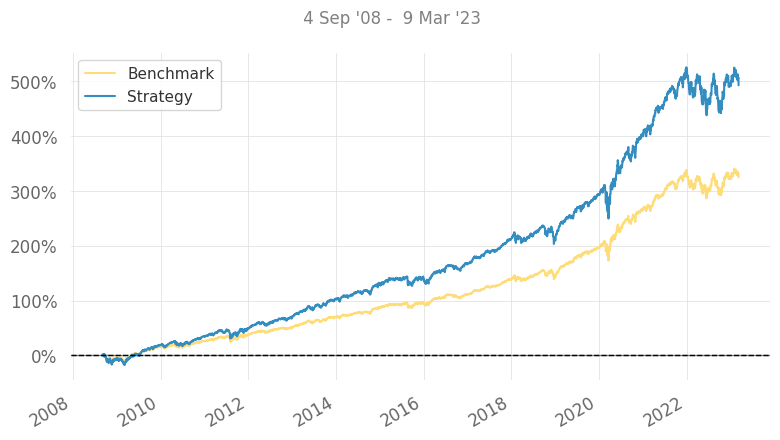
\includegraphics[width=\linewidth]{assets/long-vs-strat.png}
    \caption{Cumulative returns of the long leg of the strategy compared with the complete strategy}
    \label{fig:long-vs-strat}
\end{figure}

As it can be seen in \autoref{fig:long-vs-strat}, the overall returns of the long leg seem to be superior. However, upon closer inspection it is seen how this is only achieved through higher volatility. In fact, when matching the volatility of both these are the results:
\begin{figure}[ht]
    \captionsetup{justification=centering}
    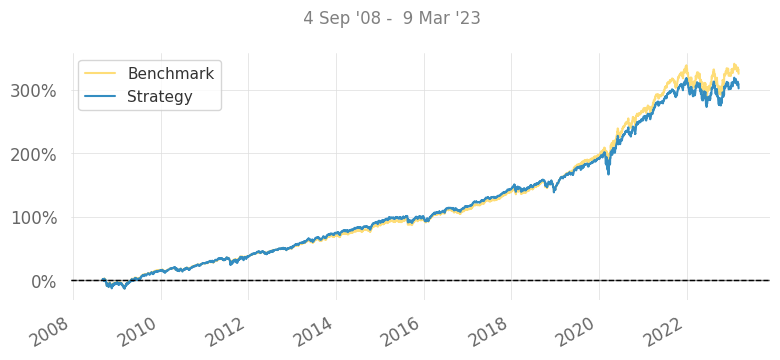
\includegraphics[width=\linewidth]{assets/long-vs-strat-vol-matched.png}
    \caption{Cumulative returns of the volatility matched long leg of the strategy compared with the strategy}
    \label{fig:long-vs-strat-vol-matched}
\end{figure}

A very interesting observation can be extracted from \autoref{fig:long-vs-strat-vol-matched}. At first, it may seem like the long leg of the strategy is just a leveraged position of the overall strategy. However, towards the end it becomes apparent how adding the short positions contributes to a very slight edge in volatility matched performance.

To see more precisely what this behaviour means in quantitative terms, the four first moments are presented in \autoref{table:main-moments-long-vs-strat}

\begin{table}[ht]
    \centering
    \begin{tabular}{rll}
        \toprule
        Metric & \multicolumn{2}{c}{Value} \\ 
        \cmidrule(lr){2-3}
            & Long leg & Strategy \\
        \midrule
        CAGR & 9.52\% & 7.65\% \\
        Annualized Volatility & 11.46\% & 8.79\% \\
        Skew & 0.04 & 0.14 \\
        Kurtosis & 6.01 & 7.9 \\
        \bottomrule
    \end{tabular}
    \caption{Main moments of the long leg of the strategy's return distribution}
    \label{table:main-moments-long-vs-strat}
\end{table}

As it could be inferred from previous observations in \autoref{fig:long-vs-strat} and \autoref{fig:long-vs-strat-vol-matched}, the mean returns and volatility of the long part of the strategy are higher than those of the strategy itself. However, looking at the third and fourth moments something more interesting comes to light. If the long portion of the strategy truly behaved like a leveraged position of the whole strategy, the skew and kurtosis would remain constant. However, the long leg exhibits a lower skew than the complete strategy, providing lower long term compound returns and more exposure to catastrophic tail negative return scenarios. Regarding the kurtosis of the distribution, it is also not the same. In this case, adding the negative positions increases this fourth moment, supposedly due to some extreme movements that are exhibited by the short leg of the strategy. This higher kurtosis, together with a positive skew, means that tail positive events are larger for the complete strategy and this facilitates having better performance with lower risk. All of this can be seen more clearly in \autoref{fig:long-vs-strat-ret-dist}.

\begin{figure}[ht]
    \captionsetup{justification=centering}
    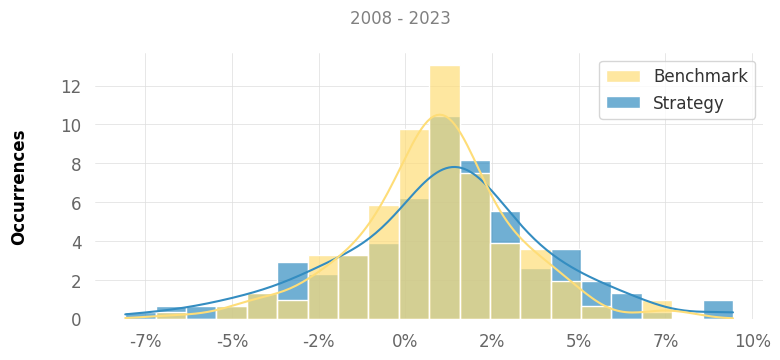
\includegraphics[width=\linewidth]{assets/long-vs-strat-ret-dist.png}
    \caption{Monthly returns distribution of the long leg of the strategy compared with the overall strategy}
    \label{fig:long-vs-strat-ret-dist}
\end{figure}

In order to understand on more practical terms what these differences in returns mean, the following metrics can be analyzed.

\begin{table}[ht]
    \centering
    \begin{tabular}{rll}
        \toprule
        Metric & \multicolumn{2}{c}{Value} \\ 
        \cmidrule(lr){2-3}
            & Long leg & Strategy \\
        \midrule
        Sharpe ratio & 1.12 & 1.16 \\
        Sortino ratio & 1.65 & 1.69 \\
        Calmar ratio & 0.51 & 0.54 \\
        Max Drawdown & -18.56\% & -14.15\% \\
        Longest Drawdown & 336 & 335 \\
        Alpha & -0.01 & -- \\
        Beta & 1.29 & -- \\
        Treynor ratio & 519.42\% & -- \\
        \bottomrule
    \end{tabular}
    \caption{Risk and risk-adjusted return metrics for the long leg of the strategy}
    \label{table:risk-adjusted-long-vs-strat}
\end{table}

By observing these metrics the similarity in perfromance between both sets of returns is again apparent. Most ratios, like the Sharpe ratio, Sortino ratio or Calmar ratio are slightly more favourable to the complete strategy, in accordance with the slightly superior volatility adjusted performance. Moreover, the leveraged looking behaviour is apparent in the beta above 1. However, as it can be seen in the rest of the ratios, this leveraged but slighly worse performance is reflected in the slightly negative alpha. 

\subsubsubsection{Short leg}

After having looked at the long leg, it is now time to look at how the performance of the short leg compares with the overall strategy. The best introduction is again the comparison of the short leg of the strategy's cumulative returns with the strategy's cumulative returns.

\begin{figure}[ht]
    \captionsetup{justification=centering}
    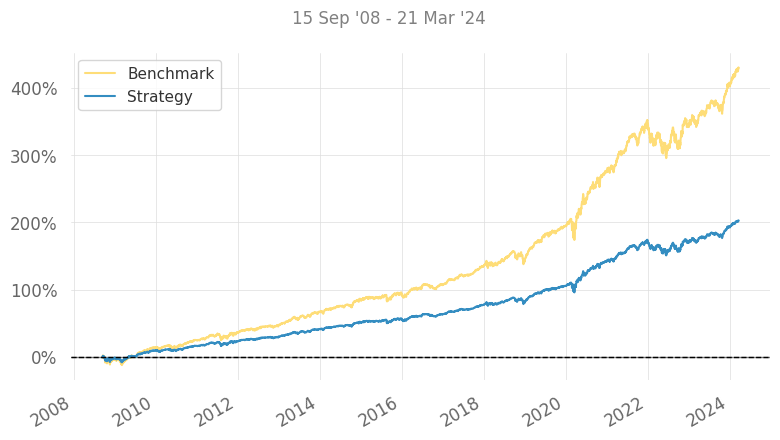
\includegraphics[width=\linewidth]{assets/short-vs-strat.png}
    \caption{Cumulative returns of the short leg of the strategy compared with the complete strategy}
    \label{fig:short-vs-strat}
\end{figure}

In this case, it can be seen how the situation seems to be the inverse one. The overall returns seem to be lower, albeit that also seems to imply a lower volatility. Referring to the volatility matched comparison is again a good reference point for checking whether these intuitions seem correct.
\begin{figure}[ht]
    \captionsetup{justification=centering}
    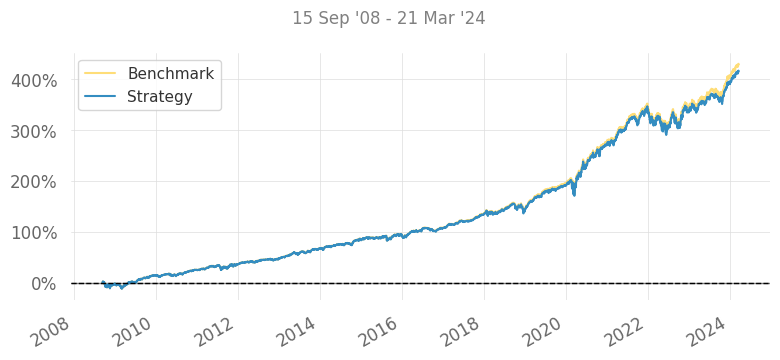
\includegraphics[width=\linewidth]{assets/short-vs-strat-vol-matched.png}
    \caption{Cumulative returns of the volatility matched short leg of the strategy compared with the strategy}
    \label{fig:short-vs-strat-vol-matched}
\end{figure}

Even though the performance seemed to be the opposite to that of the long leg -- lower performance through lower volatility -- in \autoref{fig:short-vs-strat-vol-matched} it can be seen that both are more similar than it would seem. The volatility matched performance is again very similar to that of the complete strategy, with a slight edge becoming again apparent towards the end of the period.

Referring again to the four first moments can be helpful in shedding some quantiative light.

\begin{table}[ht]
    \centering
    \begin{tabular}{rll}
        \toprule
        Metric & \multicolumn{2}{c}{Value} \\ 
        \cmidrule(lr){2-3}
            & Short leg & Strategy \\
        \midrule
        CAGR & 5.05\% & 7.65\% \\
        Annualized Volatility & 5.86\% & 8.79\% \\
        Skew & 0.14 & 0.14 \\
        Kurtosis & 7.9 & 7.9 \\
        \bottomrule
    \end{tabular}
    \caption{Main moments of the short leg of the strategy's return distribution}
    \label{table:main-moments-short-vs-strat}
\end{table}

Again, the previous observations regarding the mean returns and their volatility are confirmed. This time however, the distribution is itself much more similar to the complete strategy's one when regarding the third and fourth moments. 

The usual more practical metrics are again shown in \autoref{table:risk-adjusted-short-vs-strat}.
\begin{table}[ht]
    \centering
    \begin{tabular}{rll}
        \toprule
        Metric & \multicolumn{2}{c}{Value} \\ 
        \cmidrule(lr){2-3}
            & Short leg & Strategy \\
        \midrule
        Sharpe ratio & 1.08 & 1.16 \\
        Sortino ratio & 1.58 & 1.69 \\
        Calmar ratio & 0.53 & 0.54 \\
        Max Drawdown & -9.48\% & -14.15\% \\
        Longest Drawdown & 335 & 335 \\
        Alpha & -0.00 & -- \\
        Beta & 0.67 & -- \\
        Treynor ratio & 302.29\% & -- \\
        \bottomrule
    \end{tabular}
    \caption{Risk and risk-adjusted return metrics for the short leg of the strategy}
    \label{table:risk-adjusted-short-vs-strat}
\end{table}

As with the long leg, metrics are similar for the short leg and the complete strategy. Most ratios are again slightly favourable to the complete strategy as expected, but in contrast with the other half here the negative alpha practically disappears, demonstrating how the short leg is more representative of the whole strategy. 


\subsection{Factor regression}
Now, with a better understanding of the strategy's overall performance, how it compares to the market and to a more comparable benchmark, and how its performance is divided between the long and short legs of the pairs trading strategy, it is possible to finally delve into what the drivers of this performance are. 

\subsubsection{Primary regression}

First, a quick overview of the different factors can be seen through the correlation of the five in \autoref{fig:factors-corr-matrix}. It can be seen how the five factors are mostly uncorrelated, with the $MOM$ factor being the one with the highest correlation, specially to the $HML$ factor but also to the market excess returns. 
\begin{figure}[ht]
    \centering
    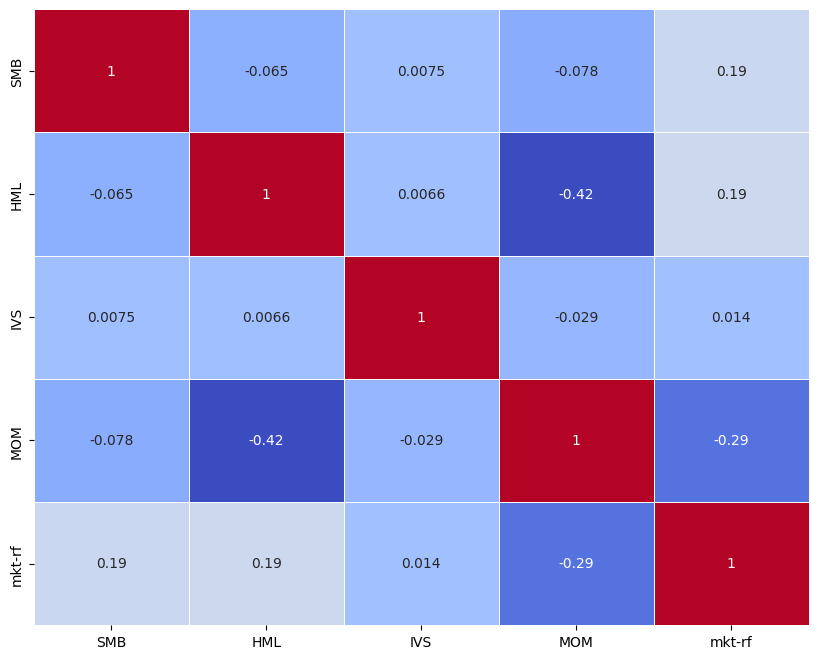
\includegraphics[width=300px]{assets/factors-corr-matrix.png}
    \caption{Correlation matrix for the five factors of the primary regression}
    \label{fig:factors-corr-matrix}
\end{figure}

\autoref{table:primary-regression-results} shows the results of the estimation of parameters for the cross section regression relative to equation \eqref{e:primary-regression}. In this regression, the whole time period of returns previously analyzed has been considered. Additionally, entity effects have been incorporated in the regression as they can serve to capture company specific information not captured by the rest of the factors as per \cite{ian_wagner_2019}. 

This main regression has been compared with other reference regressions. These follow the $CAPM$, Fama-French 3 factor model and the Carhart 4 factor model. This comparison has been performed in order to ensure the results given by the main regression are not spurious and fall in line with what more simple methods estimate for each of the drivers. Through the comparison of all regressions, a more robust result can be presented regarding the loadings for each of the factors. 

In \autoref{table:primary-regression-results} the t-statistic has also been included in parentheses below each estimated coefficient. No reference to the p-value of the t-statistic has been given as all coefficients are relevant at the $1\%$ level for all models. The $R^2$ has also been included. It can be noted how the $R^2$ increases with the number of factors as expected. The most significant jump is given by adding the two additional factors in the Fama-French model, with very little additional variance being explained by the $MOM$ and $IEP$ factors. The final model's $R^2$ stays at a moderate $2.67\%$, hinting at the idea that there may be other drivers at play needed to fully explain the performance of the strategy, hence why the secondary regression has been applied. Note that the number of observations in the regression is of 1.451.108 observations related to 398 different entities -- the 398 stocks remaining in the S\&P500 during the studied period. The F-statistic of the whole regression for the five factor model is 8004.8, demonstrating a joint significance for the model in addition to the individual significance of each of the coefficients. 

\begin{table}[ht]
    \centering
    \begin{tabular}{rcccc}
        \toprule
        Model & CAPM & FF3 & Carhart & Carhart+IEP \\ 
        \midrule
        $\alpha$ & 0.0005 & 0.0005 & 0.0005 & 0.0004 \\
                 & (98.5) & (99.0) & (98.9) & (63.3) \\[8px]
        $\beta_{mkt-rf}$ & -0.0560 & -0.0607 & -0.0631 & -0.0631 \\
                         & (-158.71) & (-166.1) & (-168.5) & (-168.5) \\[8px]
        $\beta_{SMB}$ & & 0.0783 & 0.0767 & 0.0766 \\
                      & & (106.6) & (104.2) & (104.1) \\[8px]
        $\beta_{HML}$ & & -0.0181 & -0.0249 & -0.0249 \\
                      & & (-33.7) & (-42.5) & (-42.5) \\[8px]
        $\beta_{MOM}$ & & & -0.0137 & -0.0135 \\
                      & & & (-29.4) & (-28.9) \\[8px]
        $\gamma$ & & & & 0.1085 \\
                       & & & & (9.4) \\[8px]
        \midrule
        $R^2$ & 1.71\% & 2.61\% & 2.66\% & 2.67\% \\

        \bottomrule
    \end{tabular}
    \caption{Coefficient estimations for the primary factor regression}
    \label{table:primary-regression-results}
\end{table}

Several observations can be made from the results of the coefficient estimations of the different models. The first of them is the robustness of the estimations. For all of the models, the coefficient estimations are pretty much the same for the different factor loadings. This showcases the orthogonality of the different factors, already hinted at by the low correlation shown in \autoref{fig:factors-corr-matrix}. It also indicates how there very likely is no omitted variable bias where the missing variable was being explained by one or more of the present factors and the models are correctly specified.

Regarding the coefficients themselves, it can be seen how, as already shown in the section \nameref{sec:overall-performance}, the strategy has a negative correlation to the market. It can also be seen how the strategy has a positive relation to the size factor and negative to the momentum and value factors. The negative exposure to the momentum could be expected, given how this strategy is in its essence a mean reverting strategy. However, it is interesting to see how the outperformance of low value and low size companies are key drivers of the performance of the strategy. 

Finally, regarding the Idiosyncratic Equity Volatility Premium, it can be seen how the strategy has a great exposure to this factor. Its performance seems to be greatly driven by high exposure to stocks with high idiosyncratic volatility premium, which again is to be expected as higher volatility leads to more opportunities to enter a position away from the long term equilibrium and thus more opportunities to profit when the stocks return to their cointegration equilibrium. More specifically, an increase in 1\% for the Idiosyncratic Equity Volatility Premium across stocks leads to an increase of 0.1 percentage point in the daily returns of the strategy. These companies can be found in sectors with rapid innovation, frequent regulatory changes or high sensitivity to firm-specific news, like the technology sector, or the pharmacetical or biotechnology sectors, with companies such as Tesla, Nvidia or Moderna being examples of specific stocks. 

Finally, there seems to be a consistent $\alpha$ of unexplained performance by the used five factor model. This $\alpha$ of 0.04\% in daily returns is a very significant 10.08\% in annual outperformance over the five factor benchmark model. 

\subsubsection{Secondary regression}
As it could be seen in the previous section, the five factor model used to understand the drivers of the strategy was very robust and it pointed the light at some of the key drivers of the strategy's performance. However, the low $R^2$ hints at the possibility of uncovering more of its drivers through more variables. 

In order to achieve that, the previous regression is performed on a rolling basis with quarterly data and a cross section regression is performed with company data on the different $\alpha$ obtained on those regressions. 

But first, a preliminary look at the correlation between the different factors can be useful to understand what information these may share among themselves. 

\begin{figure}[ht]
    \centering
    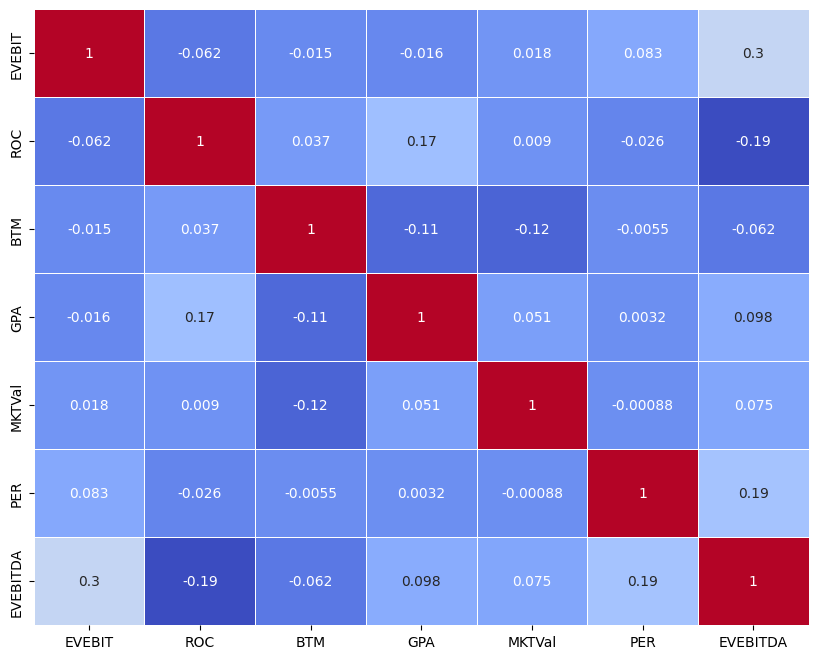
\includegraphics[width=300px]{assets/factors-secondary-corr-matrix.png}
    \caption{Correlation matrix for the seven factors of the secondary regression}
    \label{fig:factors-secondary-corr-matrix}
\end{figure}

The first thing to note in \autoref{fig:factors-secondary-corr-matrix} is the low correlation among the seven different factors, with the highest being a correlation of 30\%. This highest value is unsurprisingly that between $EVEEBIT$ and $EVEBITDA$, variables which transmit similar value related information, but which however are not as similar as the names may suggest. The next highest values are between $ROC$ and $GPA$, both profitability related metrics, and between $ROC$ and $EVEBITDA$, but even these third and seconds highest correlation pairs have a correlation of below 20\%. Most of the values are in the single digits, sign of the high orthogonality between most pairs of assets. 

The first secondary regression, with all factors indicated in the model shown in equation \eqref{eq:secondary-regression} and already presented in \autoref{fig:factors-secondary-corr-matrix}, has had the coefficients estimated on the alphas of all available quarters with the information of all available companies. The results of the estimation can be found in \autoref{table:secondary-regression-results-1}.

In this regression the $R^2$ achieved is of 1.09\%. There are 58 consecutive time periods corresponding for the 58 consecutive quarters in the studied period. The regression is jointly significant at all significance values with an F-statistic of 32.6. Again, individual entity effects are included as per \cite{ian_wagner_2019}. 
\begin{table}[ht]
    \centering
    \begin{tabular}{rccc}
        \toprule
        Coefficient & Estimation & t-statistic & p-value \\ 
        \midrule
        $\alpha$ & -0.0011 & -5.8 & 0.0000 \\
        $\gamma_{MKTVal}$ & 0.014 & 8.2 & 0.0000 \\
        $\gamma_{GPA}$ & 8.3e-5 & 0.8 & 0.3989 \\
        $\gamma_{ROC}$ & 0.0008 & 2.0 & 0.0443 \\
        $\gamma_{EVEBIT}$ & -0.0002 & -0.4 & 0.6612 \\
        $\gamma_{EVEBITDA}$ & 0.0007 & 4.1 & 0.0000 \\
        $\gamma_{PER}$ & 0.0005 & 0.8 & 0.4448 \\
        $\gamma_{BTM}$ & -0.0046 & -10.0 & 0.0000 \\
        \bottomrule
    \end{tabular}
    \caption{Coefficient estimations for the secondary factor regression}
    \label{table:secondary-regression-results-1}
\end{table}

However, even though the regression is jointly significant there are some coefficients which are not. Given the low shared information between the different factors, this is probably due to the outperformance of the strategy being unrelated to the information provided by some of these metrics. 

Through a process of iterative elimination of non significant variables, a final regression with more significant paramteters is obtained. 

\begin{table}[ht]
    \centering
    \begin{tabular}{rccc}
        \toprule
        Coefficient & Estimation & t-statistic & p-value \\ 
        \midrule
        $\alpha$ & -0.0011 & -5.9 & 0.0000 \\
        $\gamma_{MKTVal}$ & 0.014 & 8.2 & 0.0000 \\
        $\gamma_{ROC}$ & 0.0009 & 2.3 & 0.0192 \\
        $\gamma_{EVEBITDA}$ & 0.0007 & 4.1 & 0.0000 \\
        $\gamma_{BTM}$ & -0.0047 & -10.1 & 0.0000 \\
        \bottomrule
    \end{tabular}
    \captionsetup{justification=centering}
    \caption{Coefficient estimations for the secondary factor regression after iterative variable elimination}
    \label{table:secondary-regression-results-2}
\end{table}

In this final regression, all parameters are significant at all significance level, except for the Return on Capital which is singificant at the 5\% confidence level. 

The first interesting piece of information, like with Sherlock's dog, is given by what is missing. All factors that have been dropped due to their low significance -- namely Gross Profit over Assets, Enterprise Value to EBIT and Price to Earnings ratio -- can be inferred not to be drivers of the performance of the strategy. That is, those measures seem to be irrelevant to how the strategy performs, so including or removing assets based on those factors alone shouldn't have any significant impact given all other factors remain unchanged. 

According to \autoref{table:secondary-regression-results-2}, the strategy seems to outperform due to the assets with high market capitalization in the most significant way, but also due to those on the higher end of the valuation spectrum according to the $BTM$, same according to the $EVEBITDA$ and  with high profitability according to $ROC$. Note however how this could be due to sectoral preferences. The tech sector for example fits the description for all factors, so it could also be that the overperformance of the strategy is accentuated due to exposure to this sector wich has historically outperformed. This showcases the difference in the investment selection between this strategy and traditional rules-based strategies. These strategies which use fundamental factors generally tend to leave out investments in the technology sector due to having some undesirable ratios (e.g. PE ratio above the investment criteria threshold). This strategy thus lacks this bias which has burdened the performance of many such traditional strategies.
\newpage
% \input{sections/discussion}
% \newpage
\section{Conclusion}

Although pairs-trading strategies have a long history, both in academic literature and in practice, most research has been centered on developing novel strategies and improving their performance through different adaptations. There is still work to be done regarding the explainability of its returns and the driver analysis for explanatory and practical purposes. 
In this work, the already developed implementation of a cointegration based pairs-trading strategy has been modified in order to make it practical to apply it to a larger universe of assets and to improve its performance through some adaptations. During the implemented backtest more information is stored regarding the returns of the long and short leg of the strategy and the number of open positions at each timestep. A comparable benchmark based on Johansen cointegration is developed and implemented. The results of the complete strategy are examined first from a performance perspective comparing it to the market and the developed benchmark. This performance analysis is enhanced by also studying the performance of the long and short legs of the strategy independently, examining what each side contributes to the overall strategy. 
After the performance is studied, the main drivers of this performance are analysed. A factor model is developed and implemented and the returns of the strategy are used to obtain the factor loadings for said model, shedding some light on which of the factors are responsible for the studied results. After a low $R^2$ for the model fit and a significant $\alpha$ of unexplained outperformance is obtained, this $\alpha$ is resampled quarterly and a second regression on company specific disclosed data relating to valuation and profitability is performed. The results obtained through the fitting of this secondary model shed some further light on which specific financial factors contribute as drivers of the performance of the strategy. 

The implemented strategy has been shown to clearly outperform both the market and the comparable benchmark on a risk adjusted basis on pretty much all performance metrics, from financial ratios to statistic measures. It has also been shown to have a low negative beta with respect to the market and thus provide a very useful point of difersification for any market participant. Both the long and short leg of the strategy have been shown to have a very similar return profile to the overall strategy, with the long leg having higher risk and higher return performance, and the short leg having lower risk and lower returns. The combination of the two has also been demonstrated to have a better risk adjusted performance than any of the individual halves. It has also been shown how the performance seems to be unrelated to the number of open positions. 
The primary regression with the five factor model has been shown to be robust and all coefficients have been found to be highly significant. The strategy has been shown to, in addition to the negative exposure to market already mentioned, be mainly driven by the size factor and the Idiosyncratic Volatility Spread, both being significant positive drivers of the PnL. There has also been shown to be a smaller negative exposure to the momentum and value premium factors. The outperformance of this strategy relative to this model has been shown to be singificant at an annualized value of $\alpha=10.08\%$. 
The secondary regression has shown that some of the factors initially thought to be drivers of the strategy -- namely $GPA$, $EVEBIT$ and $PER$ -- were in fact not significant. The significance of the rest was shown with a more robust model reached through iterative elimination of non significant factors. The strategy's performance was shown to be favoured by exposure to companies with high market capitalization, highly profitable as measured by the Returns on Capital, and with high valuations as measured by the Enterprise Value to EBITDA and Book-to-Market ratios. 

There are still many interesting avenues for future research, both in the analysis of the performance of the strategy and the study of its main drivers. 
As for the implementation, a more realistic backtest could be implemented by including transaction costs, lending costs of the short positions, slippage, risk of margin calls, etc. This would lead to a more realistic performance backtest, although the main findings of this work are expected to remain relevant even in the light of those results. Also, more time periods and universes of assets could be analysed to ensure the robustness of the outperformance of the strategy.
Regarding the driver analysis, there is room for more explainability through the inclusion of factors different to those that have been included here, with sector exposure being a promising start. It should also be explored whether a selective filtering of the assets based on its positive drivers leads to better risk adjusted performance. It will be interesting to see how more analysis of the key drivers of pairs-trading strategies and on a deeper and more disaggregated way could lead to better performance in practice.
\newpage
\begin{appendices}
\section{Performance metrics explained}
\label{sec:performance-metrics-explained}
When studying a given asset or strategy as an investment opportunity, there are many things to consider. The investor is interested in returns, but also in risk. And risk can be measured as return volatility as in the classical portfolio optimization paper \cite{markowitz_1952}, but also in many other ways. 

In order to compare the performance of the strategy with the different benchmarks in the most complete way, several different metrics have been selected and calculated. Here, these different metrics will be explained in more depth to understand how they are calculated, what they represent and how they can be useful. 

\begin{itemize}
    \item \textbf{Sharpe ratio}: This ratio introduced by \cite{sharpe_1966} and revised in \cite{sharpe_1994} is a risk adjusted return metric that incorporates both the mean returns and the volatility of those returns. It is calculated as 
    \begin{equation}
        SR=\frac{r_a-r_f}{\sigma_{r_a-r_f}}
    \end{equation}
    where $r_a$ is the annualized mean asset returns, $r_f$ is the risk free returns and $\sigma_{r_a-r_f}$ is the volatility of the asset's excess returns. 
    It measures how much excess returns are generated per unit of risk taken.
    \item \textbf{Sortino ratio}: One of the main drawbacks of the Sharpe ratio is that for some investors the volatility of the returns may not be an accurate measure of risk. The investor tries to avoid downwards movements of the returns, but upwards movements are more than welcome. In order to solve that misrepresentation of risk by the Sharpe ratio, the Sortino ratio was developed in \cite{sortino_1994}. This ratio is also a measure of risk adjusted returns, but the risk is measured as the volatility only of the negative returns. It is calculated like
    \begin{equation}
        Sortino=\frac{r_a-r_f}{\sigma^-_a}
    \end{equation}
    where $\sigma_a^-$ is the volatility exclusively of the negative returns. 
    It measures the excess returns generated per unit of risk measured as downside volatility. 
    \item \textbf{Drawdown}: The drawdown is a measure of risk which accounts for the total loss that can be expected for the given investment. For a series of returns $r_t$ for $t=0,1,2,...T$, the drawdown at $T$ is calculated as 
    \begin{equation}
        DD_T=\frac{\text{max}\left[W_t\right]-W_T}{\text{max}\left[W_t\right]}
    \end{equation}
    where $W_t$ is the compounded wealth at time $t$ accumulated due to all previous returns. The maximum drawdown is $\text{max}\left[DD_t\right]$ across the whole investment period. It is a measure of the maximum loss the investor could have expected to have.
    \item \textbf{Calmar ratio}: This ratio was created in order to combine the risk as measured by the maximum drawdown with return information to create a risk adjusted return measure. It is calculated as 
    \begin{equation}
        Calmar=\frac{r_a}{\text{max}\left[DD_t\right]}
    \end{equation}
    This measure gives the investor a sense of how much returns can be expected per percentage point of maximum drawdown. 
    \item \textbf{Beta}: This measure introduced in the $CAPM$ model in \cite{sharpe_1964} is the same coefficient which accompanies the market excess returns factor. It is also a measure of risk and independently it is calculated as 
    \begin{equation}
        \beta=\frac{Cov\left(r_a,r_b\right)}{\sigma^2_b}
    \end{equation}
    where $Cov\left(r_a,r_b\right)$ is the covariance of the asset's returns and the benchmark's returns and $\sigma^2_b$ is the benchmark returns' variance. This $\beta$ measures the sensitivity of the asset's returns to the benchmark's returns, with a $\beta=1$ indicating that the asset moves in line with the market, $\beta=0$ indicating returns completely uncorrelated with the market and $\beta \in \left(-\inf,\inf\right)$. This is thus a measure of sistematic risk when taking the market as the benchmark.
    \item \textbf{Alpha}: While $\beta$ was a measure of risk related to the $CAPM$ model, $\alpha$ is the corresponding measure of risk adjusted returns. It is calculated as
    \begin{equation}
        \alpha=r_a-\beta r_b
    \end{equation}
    Note how this $\alpha$ is different from that of the $CAPM$ model -- although it is inspired by it -- which would be calculated as $\alpha=r_a-\left[r_f+\beta\left(r_b-r_f\right)\right]$. The difference lies in that this one is calculated with respect to a generic model benchmark. The $\alpha$ then represents the excess returns of the asset with respect to the returns excpected according to the benchmark model, given its risk as measured by $\beta$. It indicates whether the asset has outperformed the benchmark after adjusting for risk.
    \item \textbf{Treynor ratio}: This ratio introduced by Jack L. Treynor is again a metric for risk adjusted returns similar to the Sharpe ratio but using the already explained $\beta$ as a measure of risk. It is thus calculated as 
    \begin{equation}
        Treynor=\frac{r_a-r_f}{\beta}
    \end{equation}
    It shows how much additional excess returns can be expected per unit of additional systematic risk.  
\end{itemize}
\newpage
\section{Code implementation}
\label{sec:code}
The complete code used in this work has been made publicly accessible. That is, the implementation of the strategy but also all the code use to create and estimate the factor models, to obtain the alphas for the quarterly regressions, to study the performance of the strategy, etc. Even the latex version of this written document has been made accessible. All that code can be accessed via GitHub at \href{https://github.com/fcelya/long-short-pnl-drivers}{https://github.com/fcelya/long-short-pnl-drivers}. The only elements that have not been made accessible are the datasets used to run the strategy and to estimate the factor parameters. They could not be uploaded due to GitHub's limitations, and enough information has been given in \autoref{sec:data-description} for anyone to be able to recreate those datasets. 

The hope is that by making this code easily accessible, more people will be tempted to explore it, play with it and the ideas presented in this work can be further explored by the community at large. 
\end{appendices}
\newpage

\printbibliography[heading=bibintoc]
\end{document}
